%%%%%%%%%%%%%%%%%%%%%%%%%%%%%%%%%%%%%%%%%%%%%%%%%%%%%%%%%%
%
% Doctoral Thesis Template @ The University of Manchester
% LaTeX Chapter Template
% Version 1 (23/07/2020)
% Joe Crone
%
% This template is based on:
% The University of Manchester, Presentation of Thesis Policy
% Research Office Graduate Education Team
% June 2017
% http://www.regulations.manchester.ac.uk/pgr-presentation-theses/
%
%%%%%%%%%%%%%%%%%%%%%%%%%%%%%%%%%%%%%%%%%%%%%%%%%%%%%%%%%%
\documentclass[../main.tex]{subfiles}
\begin{document}

% Title
%--------------------------------------------------------
\chapter{Energy Recovery Linac Design}
\label{Energy_Recovery_Linac_Design} % to reference use \ref{ChapterTemplate}

\section{Equations of Motion in Particle Accelerators}

\subsection{Co-ordinate System}

In particle accelerators bending fields are often used to direct particles to an experimental station downstream of the particle source, and many particle accelerators re-circulate particle beams. In a circular accelerator particles are directed along an ideal trajectory named a reference orbit -- since in a re-circulated machine the trajectory is closed -- with a radius of curvature $\rho$. As bending forces are introduced, the motion of particles within an accelerator environment can best be described by a right handed rotating co-moving or curvilinear co-ordinate system \cite{wille2000physics}. The right handed curvilinear co-ordinate system is shown in Fig.~\ref{fig:accelerator_coord_system}.   

\begin{figure}[!h]
\centering
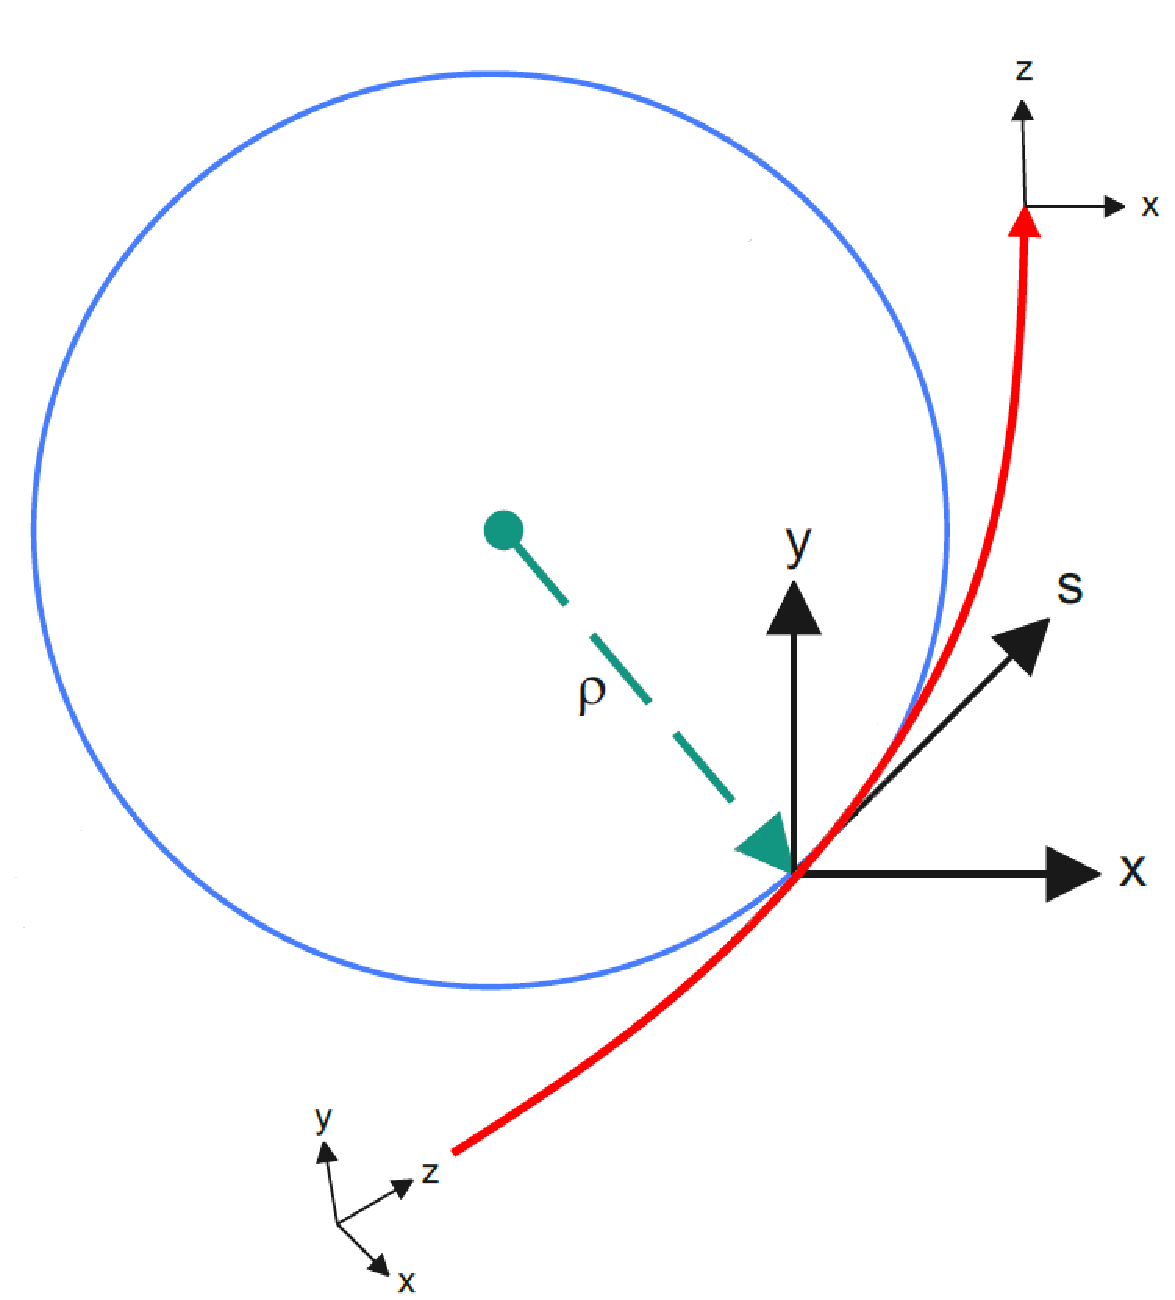
\includegraphics[width=0.6\textwidth]{Figures/Energy_Recovery_Linac_Design/Accelerator_Coord_System_fixed_V2.pdf}
\caption{The right handed curvilinear co-ordinate system used to describe particle motion in a re-circulating particle accelerator. The particles traverse around a right handed global co-ordinate system $\kappa=\left\{x,~y,~s\right\}$ with the longitudinal direction $s$, the horizontal direction $x$ and vertical direction $y$ defined around a circular reference orbit (blue) with a radius of curvature $\rho$. Particle trajectories (red)
are defined with reference to the global co-ordinate system by an attached local co-ordinate system $\iota=\left\{x,~y,~z\right\}$ where $x$ is the horizontal position, $y$ is the vertical position and $z$ is the longitudinal position with reference to the reference orbit.}
\label{fig:accelerator_coord_system}
\end{figure}

The global co-ordinate system used to describe motion in particle accelerators within this thesis is of the form $\kappa = \left\{x,y,s\right\}$, describing the global co-ordinate system where the transverse motion along the horizontal direction is in the $x$-axis and the vertical axis in $y$ is orthogonal to this and the direction of longitudinal motion $s$. Within this thesis, the $\kappa = \left\{x,y,s\right\}$ co-ordinate system is maintained in situations with no bending magnets, such as linear accelerators.  

A local co-ordinate system $\iota=\left\{x,~y,~z\right\}$, is attached to the trajectory of particles through the accelerator where the displacement of the particle from the reference orbit in the horizontal plane is given by $x$ and in the vertical plane is given by $y$, whilst the $z$ co-ordinate follows the global $s$ co-ordinate. The local co-ordinate system is useful for examining the dynamics of single particles with respect to the reference orbit. Calculations of the effects of beamline elements, such as magnets, upon the particle beam are also typically conducted in the local co-ordinate system.

\subsection{Magnetic Fields in Particle Accelerators}

The motion of a charged particle in an electromagnetic field is given by the Lorentz force 
\begin{equation}
\overrightarrow{F} = q\left(\overrightarrow{E}+\overrightarrow{v}\times\overrightarrow{B}\right),
\label{eq:Lorentz_force}    
\end{equation}
where $q$ is the charge of the particle with velocity vector $\overrightarrow{v}$, subject to an electric field $\overrightarrow{E}$ and magnetic field $\overrightarrow{B}$. When an elementary particle is acted upon solely by a magnetic field ($\overrightarrow{E}=0$), as common in an accelerator magnet, the Lorentz force (Eq.~\ref{eq:Lorentz_force}) can be re-cast into a more appropriate form using the time $t$ and the local  co-ordinate system in Fig.~\ref{fig:accelerator_coord_system}
\begin{equation}
\frac{d^{2}\iota}{dt^{2}} = \frac{e}{\gamma m}\left(\overrightarrow{v}\times\overrightarrow{B}\right)
\label{eq:displacement_Lorentz}    
\end{equation}
where $e$ is the elementary charge of the particle, $m$ is its rest mass and
\begin{equation}
\gamma = \frac{1}{\sqrt{1-\beta^{2}}} = \frac{E+m}{m},
\label{eq:Lorentz_factor}    
\end{equation}
is the Lorentz factor, where $\beta = v/c$ is the Lorentz speed factor and $E$ is the kinetic energy of the particle. Note that, unless explicitly stated, the ultra-relativistic approximation $pc = \sqrt{E^{2}-m^{2}c^{4}} \approx E$, valid for particles with $E \gg mc^{2}$ is used throughout this thesis as the particle energies discussed consistently satisfy this approximation.   

Since this thesis is concerned with re-circulated accelerators, particles typically require bending within the horizontal $x$ plane. To illustrate particle motion in a bending system, using the local co-ordinate system in Fig.~\ref{fig:accelerator_coord_system}, we consider a homogenous vertical magnetic field $B_{y}$ produced by a magnet with infinite pole width acting upon a charged particle of momentum $p_{0}$ (in convenient units of \si{\electronvolt}$/c$) to provide a bending radius of $\rho$ given by
\begin{equation}
\frac{1}{\rho} = \frac{eB_{y}}{p_{0}} = k_{0},
\label{magnet_bending_radius}    
\end{equation}
where $k_{0}$ is the normalised field strength of the magnet -- named a dipole magnet -- with no transverse co-ordinate dependence of the field. A dipole is classified as a zeroth-order magnet ($n=0$), where magnets have normalised field strengths $k_{n}$. The magnetic beam rigidity $B\rho$ is thus defined as
\begin{equation}
B\rho = \frac{p_{0}}{e},
\label{eq:magnetic_beam_rigidity}    
\end{equation}
and the bending angle $\alpha_{0}$ can be defined with reference to the magnetic beam rigidity
\begin{equation}
\alpha_{0} = \frac{\int B_{y} ds}{B\rho} = \frac{L_{eff}}{\rho}, 
\label{eq:dipole_bending_angle}    
\end{equation}
where the vertical magnetic field (dipole field) is integrated over the effective longitudinal distance traversed by the particle in the field $L_{\mathrm{eff}}$.

Accelerators are typically concerned with ensembles of particles -- named beams -- which can be transversely distributed around the ideal reference orbit (displaced horizontally or vertically from the reference orbit) due to their natural divergence. Therefore, a restorative focusing force is required to counter the natural divergence of these particles. Within accelerators a quadrupole magnet, consisting of four alternating equidistant (from the pole centre) poles, is typically used to provide the required focusing field. Quadrupoles have a transverse linearly varying magnetic field that increased in strength with distance from the pole centre. A quadrupole is a classified as a first order magnet ($n=1$). An azimuthal field gradient of the form $g = B_{\phi}/dr$ is provided, with $r$ the radial distance from the pole centre. The scalar potential of such a quadrupole field has the form
\begin{equation}
V = -gxy,
\label{eq:quadrupole_potential}    
\end{equation}
where the partial derivatives form the linearly varying magnetic fields
\begin{align}
B_{x} &= -\frac{\partial V}{\partial x} = gy, \nonumber\\
B_{y} &= -\frac{\partial V}{\partial y} = gx.
\end{align}
Therefore, using the same formalism as (Eq.~\ref{eq:dipole_bending_angle}), the focusing angle $\alpha_{1}$ of a quadrupole can be generalised to
\begin{equation}
\alpha_{1} = \frac{e}{p_{0}}grL_{\mathrm{quad}} = -k_{1}rL_{quad},
\label{eq:quadrupole_focusing_angle}    
\end{equation}
where $L_{\mathrm{quad}}$ is the effective field length of the quadrupole magnet and the normalised quadrupole gradient $k_{1}$ becomes
\begin{equation}
k_{1} = \frac{e}{p_{0}}g.
\label{eq:quadrupole_normalised_gradient}
\end{equation}
Quadrupole focusing is analogous to focusing with an optical lens, however a lens focuses simultaneously in all transverse directions whereas a quadrupole that is focusing in the horizontal plane is defocusing in the vertical plane. In the standard defined right handed local co-ordinate system (see Fig.~\ref{fig:accelerator_coord_system}), when $k_{1} > 0$, the quadrupole is horizontally focusing (vertically defocusing) and when $k_{1} < 0$, the quadrupole is vertically focusing (horizontally defocusing). Consequently, with the transverse variation in focusing behaviour, a quadrupole can not be considered a true `magnetic lens' however, taking inspiration from ray optics, the focal length of a quadrupole $f_{\mathrm{quad}}$ can be described as
\begin{equation}
\frac{1}{f_{\mathrm{quad}}} = k_{1}l_{\mathrm{quad}}.
\label{eq:focal_length_quadrupole}    
\end{equation}
The similarities between an optical lens and a quadrupole are highlighted in Fig.~\ref{fig:quad_doublet}, which shows a simple focusing defocusing scheme -- the quadrupole doublet. Though focusing and defocusing occur simultaneously in a quadrupole, overall focusing can be achieved by two properly placed quadrupoles.  

\begin{figure}[!h]
\centering
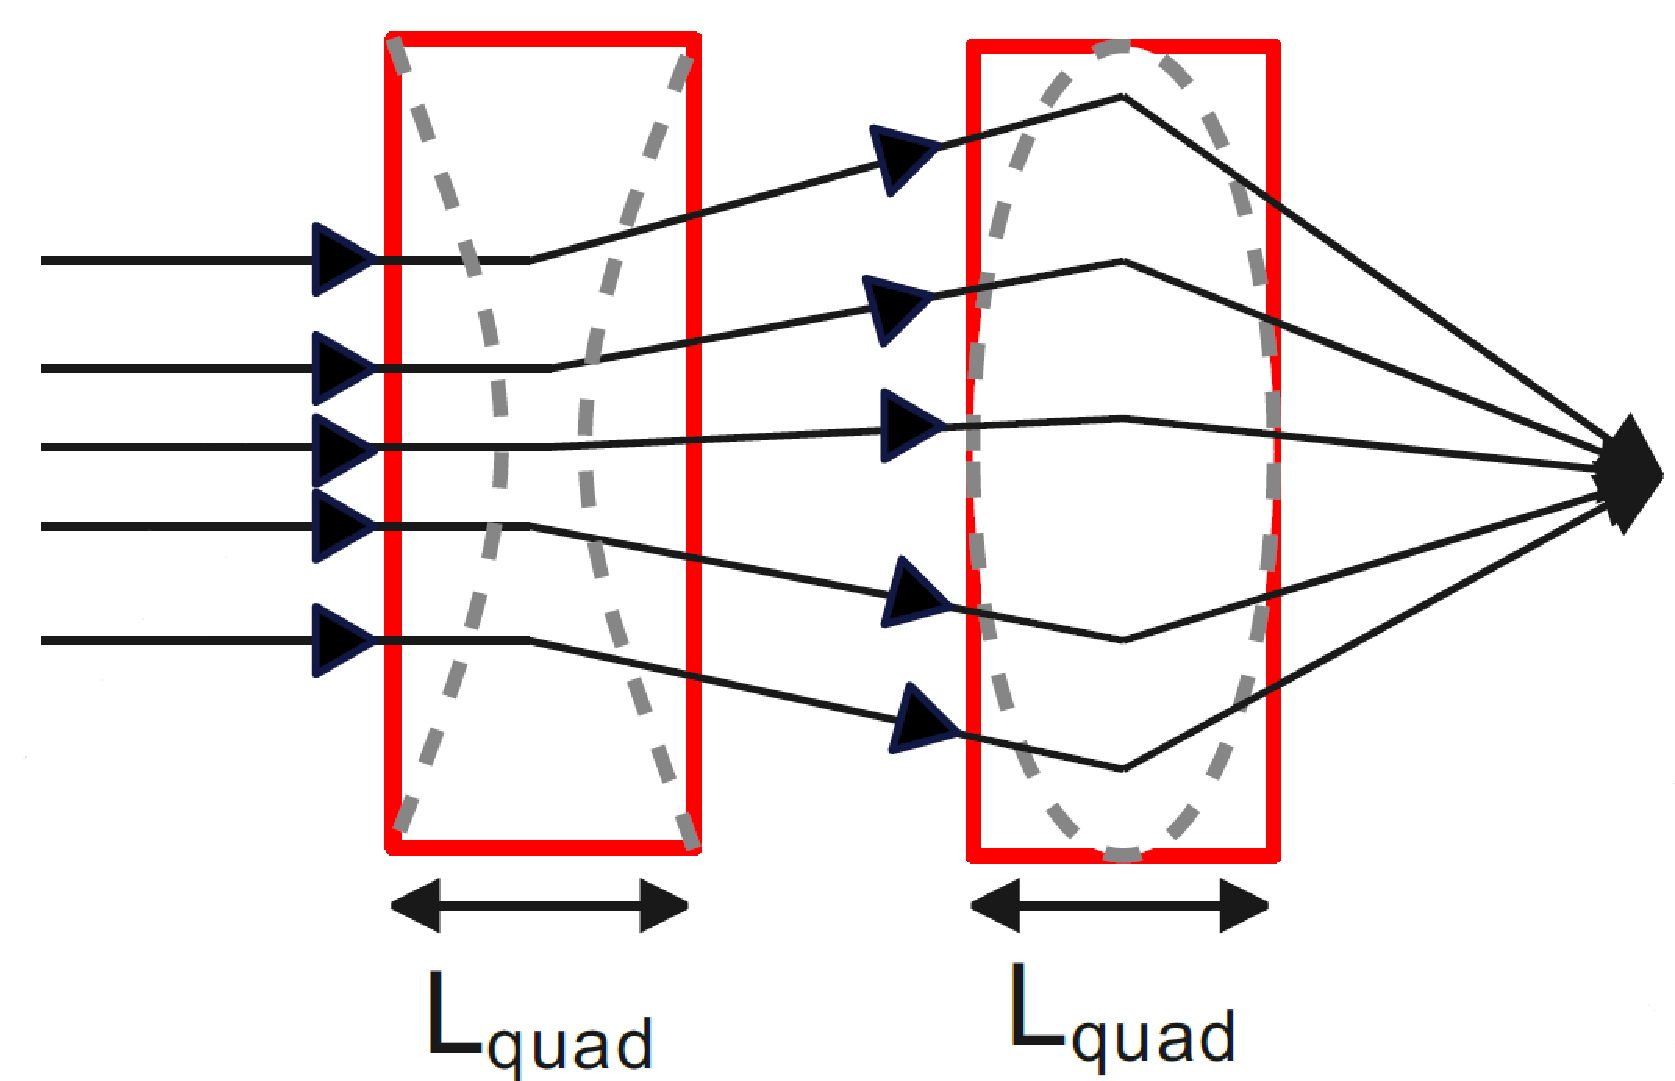
\includegraphics[width=0.7\textwidth]{Figures/Energy_Recovery_Linac_Design/Quad_Doublet_fixed_V2.pdf}
\caption{Particle trajectories (black) through a quadrupole (red) doublet consisting of a defocusing quadrupole followed by focusing quadrupole. Trajectories are bent similar to rays in conventional optics to achieve a focus.}
\label{fig:quad_doublet}
\end{figure}

The computation of the magnetic field of an arbitrary $n$th order magnet typically uses a multipole expansion of the scalar potential of the magnetic field, which for convenience is presented in cylindrical polar co-ordinates \cite{shepherd2016magnet}
\begin{equation}
V = \sum_{n=0}^{\infty} J_{n+1}r^{n+1}\cos\left[\left(n+1\right)\theta\right]+K_{n+1}r^{n+1}\sin\left[\left(n+1\right)\theta\right],
\label{eq:multipole_scalar_potential}    
\end{equation}
where $n \geq 0$ is the order of the magnet, $\theta$ is the polar angle from the horizontal plane  $x$--$z$ plane, and the coefficients $J_{n+1}$ and $K_{n+1}$ relate to the geometry of the magnet and its normalised field strength. For example, a quadrupole magnet ($n=1$) with $K_{2}=0$ is a skew quadrupole rotated 90\si{\degree} around the pole axis and with $J_{2}=0$ a normal quadrupole field  is obtained. The corresponding magnetic flux density of the magnet can be calculated for the radial $B_{r}$ or polar angle $B_{\theta}$ case by    
\begin{align}
B_{r} &= -\frac{\partial V}{\partial r}, & B_{\theta} &= -\frac{\partial V}{\partial \theta},
\label{eq:multipole_magnetic_field_cylindrical}    
\end{align}
and similarly in Cartesian co-ordinates, with proper transformation, the magnetic flux density in each transverse plane is
\begin{align}
B_{x} &= -\frac{\partial V}{\partial x}, & B_{y} &= -\frac{\partial V}{\partial y}.
\label{eq:multipole_magnetic_field_cartesian}
\end{align}
The normalised field gradient of an $n$th order magnet is generalised to
\begin{equation}
k_{n} = \frac{e}{p_{0}}\frac{\partial^{n} B_{y}}{\partial x^{n}}.
\label{eq:multipole_normalised_field_gradient}    
\end{equation}
For example, for a sextupole magnet ($n=2$) with 6 poles the magnetic flux density is given by
\begin{align}
B_{x} &= k_{2}xy, \nonumber \\
B_{y} &= \frac{k_{2}}{2}\left(x^{2}-y^{2}\right),
\label{eq:sextupole_magnetic_field}    
\end{align}
wiith the normalised field gradient given by 
\begin{equation}
k_{2} = \frac{e}{p_{0}}\frac{\partial^{2}B_{y}}{\partial x^{2}}.
\label{eq:sextupole_field_gradient}    
\end{equation}

A magnet may have more than a single order field simultaneously. For example, a magnet utilising both linear fields (dipole and quadrupole fields) can be constructed -- named a combined function magnet -- which combines dipole bending and a quadrupole focusing field components. A combination of quadrupole and dipole fields is achieved by offsetting the pole centre of a quadrupole from the reference trajectory or by linearly varying the vertical spacing between magnetic poles transversely across the pole face of a dipole magnet. The former strategy is employed in the CBETA ERL FFA return loop, an accelerator explained in more detail in Chapter~\ref{CBETA_Inverse_Compton_Scattering_Source_Design}. The transverse magnetic field of a combined function dipole--quadrupole magnet, bending in the horizontal plane, is given by 
\begin{align}
B_{x} &= \frac{p_{0}}{e}k_{1}y, \nonumber\\
B_{y} &= \frac{p_{0}}{e}\left(k_{0}+k_{1}x\right).
\label{eq:combined_function_field}    
\end{align}

\subsection{Linear Equations of Motions}
\label{sec:equations_of_motion}

\textcolor{blue}{**RE-DO THIS LATER - BIT COMPLICATED**}

The linear equations of motion for a particle follow the derivation of Rossbach and Schm\"{u}ser \cite{rossbach1993basic} and K. Willie \cite{wille2000physics}, using the co-ordinate system presented in Fig.~\ref{fig:accelerator_coord_system}. An equation of particle motion due to the Lorentz force (Eq.~\ref{eq:Lorentz_force}) is developed for the co-ordinate system which rotates due to bending forces, which we limit to the horizontal $x$--$s$ plane. We define the position vector of a particle at an arbitrary point in it's trajectory, in the global cylindrical co-ordinate system $\left\{r,\alpha,z\right\}$ as
\begin{equation}
\boldsymbol{R} = \boldsymbol{R}_{0} + r\boldsymbol{u}_{r} + z\boldsymbol{u}_{z},    
\label{eq:particle_position_vector}
\end{equation}
where $R_{0}$ is the distance of the particle from an arbitrary origin point and $\boldsymbol{u}_{r}$, $\boldsymbol{u}_{\alpha}$, $\boldsymbol{u}_{z}$ are unit vectors describing the motion of the particle. Assuming a small variation in azimuthal angle $d\theta$, the relations between the unit vectors become
\begin{align}
\frac{d\boldsymbol{u}_{r}}{d\alpha} &= \boldsymbol{u}_{\alpha}, & \frac{d\boldsymbol{u}_{\alpha}}{d\alpha} &= -\boldsymbol{u}_{r}, & \frac{d\boldsymbol{u}_{z}}{d\alpha} &= 0.
\label{eq:unit_vector_angular_derivatives}    
\end{align}
The velocity of the particle is given by
\begin{align}
\frac{d\boldsymbol{R}}{dt} &= \frac{dr}{dt}\boldsymbol{u}_{r}+r\frac{d\boldsymbol{u}_{r}}{dt} +\frac{dz}{dt}\boldsymbol{u}_{z}, \nonumber \\
\frac{d\boldsymbol{R}}{dt} &= \frac{dr}{dt}\boldsymbol{u}_{r} + r\frac{d\alpha}{dt}\boldsymbol{u}_{\alpha} + \frac{dz}{dt}\boldsymbol{u}_{z},
\label{eq:unit_vector_velocity}    
\end{align}
and differentiating within respect to time, the acceleration becomes
\begin{equation}
\frac{d^{2}\boldsymbol{E}}{dt^{2}} = \left(\frac{d^{2}r}{dt^{2}}-r\frac{d^{2}\alpha}{dt^{2}}\right)\boldsymbol{u}_{r} + \left(2\frac{dr}{dt}\frac{d\alpha}{dt}\right)\boldsymbol{u}_{\alpha} + \frac{d^{2}z}{dt^{2}}\boldsymbol{u}_{z},
\label{eq:unit_vector_acceleration}    
\end{equation}
the first part of the $\boldsymbol{u}_{r}$ term describes the effect of the variation of bending on the acceleration and the second part relates to the centrifugal acceleration of the particle. The force of the particle of mass $m$, using the acceleration (Eq.~\ref{eq:unit_vector_acceleration}), can be equated with the Lorentz force (Eq.~\ref{eq:Lorentz_force}) of the magnetic field due to the accelerator magnets ($\overightarrow{E}=0$)
\begin{equation}
m\frac{d^{2}\boldsymbol{R}}{dt^{2}}=-e\left(\overightarrow{v}\times\overightarrow{B}\right),
\label{eq:Lorentz_particle_equating_forces}
\end{equation}
which, by describing the magnetic flux density vector in cylindrical co-ordinates $\overightarrow{B} = \left(B_{r},B_{\alpha},B_{z}\right)$, can be expanded to
\begin{equation}
m\frac{d^{2}\boldsymbol{R}}{dt^{2}} = -e\left[\left(r\frac{d\alpha}{dt}B_{z}-\frac{dz}{dt}B_{\alpha}\right)\boldsymbol{u}_{r}+\left(\frac{dz}{dt}B_{r}-\frac{dr}{dt}B_{z}\right)\boldsymbol{u}_{\alpha}+\left(\frac{dr}{dt}B_{\alpha}-r\frac{d\alpha}{dt}B_{r}\right)\boldsymbol{u}_{z}\right].
\label{eq:Lorentz_particle_equating_forces_expanded}    
\end{equation}
Assuming that $B_{\alpha}=0$, as there is no longitudinally applied magnetic field -- as this would be in the direction of motion of the particle -- we obtain a set of two differential equations
\begin{align}
m\left(\frac{d^{2}r}{dt^{2}}-r\frac{d^{2}\alpha}{dt^{2}}\right)=-er\frac{d\alpha}{dt}B_{z},
\label{eq:radial_differential_equation} \\
m\frac{d^{2}z}{dt^{2}}=-er\frac{d\alpha}{dt}B_{r}.
\label{eq:angular_differential_equation}
\end{align}
Assuming a combination of focusing and bending magnets within the accelerator, we approximate these fields by using a the field of a combined function magnet (Eq.~\ref{eq:combined_function_field}). The defined field of a combined function magnet (Eq.~\ref{eq:combined_function_field}) in the local co-ordinate system can be simply equated to the field in the global cylindrical co-ordinate system  because the radial direction of the global co-ordinate system is the same as the horizontal $x$ direction of the local co-ordinate system and the vertical $y$ local co-ordinate direction is analogous to the global $z$ direction. The equivalence of the fields in each co-ordinate system can be expressed as
\begin{align}
B_{r} = B_{x} &= \frac{p_{0}}{e}k_{1}y, \\
B_{z} = B_{y} &= \frac{p_{0}}{e}\left(k_{0}+k_{1}x\right),
\label{eq:equivalent_combined_function_field}
\end{align}
Substituting the combined function magnetic flux density (Eq.~\ref{eq:equivalent_combined_function_field}) into the differential equations (Eqs.~\ref{eq:radial_differential_equation}, \ref{eq:angular_differential_equation}) and making the substitution $r=\rho+x$ to account for varying transverse position around the reference orbit yields
\begin{align}
m\left(\frac{d^{2}x}{dt^{2}}-\left(p+x\right)\frac{d^{2}\alpha}{dt^{2}}\right) &=-p_{0}\left(\rho+x\right)\frac{d\alpha}{dt}\left(k_{0}+k_{1}\right), 
\label{eq:horizontal_differential_equation}\\   
m\frac{d^{2}z}{dt^{2}} &= -p_{0}\left(\rho+x\right)\frac{d\alpha}{dt}k_{1}z.
\label{eq:vertical_differential_equation}
\end{align}
The azimuthal component of the velocity has the form
\begin{equation}
v_{\alpha} = \left(\rho+x\right)\frac{d\alpha}{dt},
\label{eq:azimuthal_velocity}    
\end{equation}
which is typically much larger than the radial and vertical component ($v_{\alpha}\gg v_{r},~v_{z}$), which enables the approximation $v\approx v_{\alpha}$ that the azimuthal velocity is the velocity of the particle. Using this approximation a series of variables can be replaced using
\begin{align}
s&=vt, & \frac{d^{2}x}{dt^{2}} &= v^{2}\frac{d^{2}x}{ds^{2}},
\label{eq:velocity_approximation_replacing_variables}    
\end{align}
which can then be used to re-cast (Eqs.~\ref{eq:horizontal_differential_equation}, \ref{eq:vertical_differential_equation}) to obtain
\begin{align}
\frac{d^{2}x}{ds^{2}} &= -\frac{p_{0}}{mv}\frac{1}{\rho+x}\left(k_{0}+k_{1}x\right),
\label{eq:horizontal_recast_differential_equation} \\
\frac{d^{2}z}{ds^{2}} &= -\frac{p_{0}}{mv}k_{1}z.
\label{eq:vertical_recast_differential_equation}
\end{align}
Variation in the design momentum $\Delta p$ is introduced via
\begin{equation}
mv = p = p_{0}\left(1+\frac{\Delta p}{p_{0}}\right),
\label{eq:design_momentum_variation}    
\end{equation}
which means the transverse $r$ co-ordinate can be re-cast, when $\rho \gg x$, as
\begin{equation}
\frac{1}{r}\approx \frac{1}{\rho}\left(1-\frac{x}{\rho}\right). 
\label{eq:r_rho_relation}
\end{equation}
By introducing the momentum variation (Eq.~\ref{eq:design_momentum_variation}) and the approximation of the radial component (Eq.~\ref{eq:r_rho_relation}), the equations of motion can be shown in their familiar form \cite{rossbach1993basic,wille2000physics}
\begin{align}
\frac{d^{2}x}{ds^{2}} +\left(k_{1}+\frac{1}{\rho^{2}}\right)x &= \frac{1}{\rho}\frac{\Delta p}{p_{0}},
\label{eq:horizontal_equation_of_motion} \\
\frac{d^{2}z}{ds^{2}} - k_{1}z &= 0,
\label{eq:vertical_equation_of_motion}
\end{align}
where the focusing terms of the equations of motion, arising from the focusing component $k_{1}$ and the bending component $1/\rho^{2}$ can be combined into a single term
\begin{align}
\frac{d^{2}x}{ds^{2}} + K_{x}x &= \frac{1}{\rho}\frac{\Delta p}{p_{0}},
\label{eq:horizontal_equation_of_motion_simplified} \\
\frac{d^{2}z}{ds^{2}} + K_{z}z &= 0,
\label{eq:vertical_equation_of_motion_simplified}
\end{align}
where
\begin{align}
K_{x} &= k_{1} + \frac{1}{\rho^{2}}. \nonumber\\
K_{z} &= -k_{1}.
\label{eq:focusing_equation_of_motion}    
\end{align}
The equations of motion (Eqs.~\ref{eq:horizontal_equation_of_motion_simplified}, \ref{eq:vertical_equation_of_motion_simplified}) have the form of a harmonic oscillator.

Solutions to the equations of motion (Eqs.~\ref{eq:horizontal_equation_of_motion_simplified}, \ref{eq:vertical_equation_of_motion_simplified}) can therefore be found by linear combinations of sine and cosine terms which, for the focusing case ($K>0$) have the form
\begin{align}
C\left(s\right) &= \cos\left(\sqrt{K}s\right), \nonumber\\
S\left(s\right) &= \frac{1}{\sqrt{K}}\sin\left(\sqrt{K}s\right),
\label{eq:focusing_solution_equation_of_motion}
\end{align}
and for the defocusing case ($K<0$) become
\begin{align}
C\left(s\right) &= \cosh\left(\left|K\right|s\right), \nonumber \\
S\left(s\right) &= \frac{1}{\sqrt{\left|K\right|}}\sinh\left(\left|K\right|s\right).
\label{eq:defocusing_solution_equation_of_motion}    
\end{align}
Generalising for each plane $u\left(s\right)\equiv x\left(s\right) \parallel z\left(s\right)$ the solutions become
\begin{align}
u\left(s\right) &= aC\left(s\right) + bS\left(s\right) + \frac{\Delta p}{p_{0}}D\left(s\right), \nonumber \\
u'\left(s\right) &= aC'\left(s\right) + bS'\left(s\right) + \frac{\Delta p}{p_{0}}D\left(s\right),
\label{eq:generalised_solution}
\end{align}
where $D\left(s\right)$ is the dispersion function (see Section~\ref{sec:dispersion_off_momentum_particles}), which accounts for the effect of momentum on particle trajectories and $a$, $b$ are coefficients related to the initial conditions of the particles. Commonly, for convenience, the solution (Eq.~\ref{eq:generalised_solution}) to the equations of motion is expressed in matrix formalism
\begin{equation}
\begin{pmatrix}
u\left(s\right) \\
u'\left(s\right) \\
\Delta p/p_{0}
\end{pmatrix} = 
\begin{pmatrix}
C\left(s\right) & S\left(s\right) & D\left(s\right) \\
C'\left(s\right) & S'\left(s\right) & D'\left(s\right) \\
0 & 0 & 1
\end{pmatrix}
\begin{pmatrix}
u\left(s_{0}\right) \\
u'\left(s_{0}\right) \\
\Delta p/p_{0}
\end{pmatrix},
\label{eq:general_solution_matrix}    
\end{equation}
where $s_{0}$ is the initial longitudinal position of the particle.

\section{Transport Matrices} 

Previously, the solution to the equations of motion with a periodically focusing and bending particle accelerator (Eqs.~\ref{eq:horizontal_equation_of_motion_simplified}, \ref{eq:vertical_equation_of_motion_simplified}) have been derived and presented using a matrix formalism (Eq.~\ref{eq:general_solution_matrix}). Considering the dynamics in both transverse planes ($x$ and $y$) simulataneously, the effect of momentum deviation from the design momentum $\Delta p/p_{0}$ and accounting for the longitudinal position of the particle $s=ct$, with $t$ the time-of-flight of the particle, six co-ordinates are required to describe the motion. Therefore, the position of a particle in an accelerator is adequately described using a 6D vector 
\begin{equation}
\boldsymbol{X} = 
\begin{bmatrix}
x \\
x' \\
y \\
y' \\
ct \\
\Delta p/p
\end{bmatrix},
\label{eq:6D_vector}
\end{equation}
where $x$, $y$, $ct$ are the horizontal, vertical and longitudinal positions of the particle and $x'$, $y'$ are the divergence of the particle in either plane.

The beamline of an accelerator traversed by a particle consists of a series of magnetic elements, such as dipoles, quadrupoles etc. where their effect on the particle collectively can be described by a $6~\times~6$ transform or transport matrix $\boldsymbol{R}$ (to first order). With an initial particle vector $\boldsymbol{X}_{0}$ of the form (Eq.~\ref{eq:6D_vector}), the transport matrix can relate the initial state of a particle to its final state $\boldsymbol{X}$, where a distance $s-s_{0}$ is traversed
\begin{equation}
\boldsymbol{X}_{1} = \boldsymbol{R}\boldsymbol{X}_{0}.
\label{eq:overall_transport_matrix}
\end{equation}
The transport matrix is typically constructed from a series of magnetic elements and drift spaces, therefore the transport matrix has the form
\begin{equation}
\boldsymbol{R} = \boldsymbol{R}_{n}\boldsymbol{R}_{n-1}\ldots\boldsymbol{R_{1}},
\label{eq:subseries_transport_matrix}    
\end{equation}
where $R_{n}$ are the transport matrices of each individual element. A periodic beamline is constructed from a subset of repeated  elements, named a cell, which is repeated several times. Within the following subsections, the individual transport matrices of linear magnets are described. 

\subsection{Drift Space}

A drift space within an accelerator is a section of beamline in which no magnets are placed -- the particles traverse through a vaccuum chamber subject to negligible external magnetic forces. The beam is not bent or focused, therefore the position of the particles transforms only due to their divergence. For example, in the horizontal direction $x_{1} = x_{0} + L_{\mathrm{drift}}x_{0}'$, with $L_{\mathrm{drift}}$ the length of the drift space. The $\boldsymbol{R}$ matrix for a drift space is consequently given by  
\begin{equation}
\boldsymbol{R}_{\mathrm{drift}} =
\begin{pmatrix}
1 & L_{\mathrm{drift}} & 0 & 0 & 0 & 0 \\
0 & 1 & 0 & 0 & 0 & 0 \\
0 & 0 & 1 & L_{\mathrm{drift}} & 0 & 0 \\
0 & 0 & 0 & 1 & 0 & 0 \\
0 & 0 & 0 & 0 & 1 & 0 \\
0 & 0 & 0 & 0 & 0 & 1
\end{pmatrix}.
\label{eq:drift_matrix}    
\end{equation}

\subsection{Quadrupole Magnet}

The quadrupole element focuses a particle over a magnetic length $L_{\mathrm{quad}}$ identical to the width of the magnet for a hard-edged field model where the field terminates at the end of the magnet yoke. Quadrupole focusing in one plane and defocusing in another plane, as shown in (Eqs.~\ref{eq:focusing_solution_equation_of_motion}, \ref{eq:defocusing_solution_equation_of_motion}), is encapsulated within the $\boldsymbol{R}$ matrix of this element. The quadrupole has a normalised field strength $k_{1}$ (Eq.~\ref{eq:quadrupole_normalised_gradient}), which is used to characterise the magnitude of the focusing in the transport matrix. The $\boldsymbol{R}$ matrix for a quadrupole is given by

\begin{equation}
\resizebox{\columnwidth}{!}{
\boldsymbol{R}_{\mathrm{quad}} = 
\begin{pmatrix}
\cos\left(\sqrt{k_{1}}L_{\mathrm{quad}}\right) & \frac{1}{\sqrt{k_{1}}}\sin\left(\sqrt{k_{1}}L_{\mathrm{quad}}\right) & 0 & 0 & 0 & 0 \\
-\sqrt{k_{1}}\sin\left(\sqrt{k_{1}}L_{\mathrm{quad}}\right) & \cos\left(\sqrt{k_{1}}L_{\mathrm{quad}}\right) & 0 & 0 & 0 & 0\\
0 & 0 & \cosh\left(\sqrt{k_{1}}L_{\mathrm{quad}}\right) & \frac{1}{\sqrt{k_{1}}}\sinh\left(\sqrt{k_{1}}L_{\mathrm{quad}}\right) & 0 & 0 \\
0 & 0 & \sqrt{k_{1}}\sinh\left(\sqrt{k_{1}}L_{\mathrm{quad}}\right) &  \cosh\left(\sqrt{k_{1}}L_{\mathrm{quad}}\right) & 0 & 0\\
0 & 0 & 0 & 0 & 1 & 0\\
0 & 0 & 0 & 0 & 0 & 1
\end{pmatrix}.}
\label{eq:quadrupole_matrix_thick}    
\end{equation}
The $\boldsymbol{R}$ matrix of a quadrupole (Eq.~\ref{eq:quadrupole_matrix_thick}) can be simplified using the thin lens approximation, which states that the focal length of the quadrupole (Eq.~\ref{eq:focal_length_quadrupole}) is much larger than the magnetic length of the quadrupole $f \gg L_{\mathrm{quad}}$. The transport matrix for a thin lens quadrupole becomes
\begin{equation}
\boldsymbol{R}_{\mathrm{quad, thin}} = 
\begin{pmatrix}
1 & 0 & 0 & 0 & 0 & 0 \\
-\sqrt{k_{1}}\sin\left(\sqrt{k_{1}}L_{\mathrm{quad}}\right) & 1 & 0 & 0 & 0 & 0 \\
0 & 0 & 1 & 0 & 0 & 0 \\
0 & 0 &  \sqrt{k_{1}}\sinh\left(\sqrt{k_{1}}L_{\mathrm{quad}}\right) & 1 & 0 & 0 \\
0 & 0 & 0 & 0 & 1 & 0 \\
0 & 0 & 0 & 0 & 0 & 1 
\end{pmatrix}.
\label{eq:quadrupole_matrix_thin}    
\end{equation}
The thin lens approximation is describing a quadrupole field in the zero-length regime i.e $L_{\mathrm{quad}}\rightarrow 0$\cite{rossbach1993basic}.

\subsection{Dipole Magnet}

Here we assume a sector dipole magnet with no focusing terms, where the magnetic field is homogenous transversely throughout the dipole magnet. The sector dipole is assumed to have exit and entrance pole faces, defined by the angles $\beta_{1}$ and $\beta_{2}$ respectively, that are perpendicular to the direction of the reference orbit ($\beta_{1}=0$, $\beta_{2}=0$). A diagram of a sector dipole is shown in Fig.~\ref{fig:dipole_magnet_diagram}.

\begin{figure}[!h]
\centering
\includegraphics[width=0.8\textwidth]{Figures/Energy_Recovery_Linac_Design/Dipole_magnet_V2_fixed.pdf}
\caption{Bent trajectory of a particle (red) as it traverses a sector dipole of magnetic length $L_{\mathrm{dip}}$, with radius of curvature $\rho$ and bend angle $\alpha_{1}$ in the horizontal $x$--$s$ plane. The angles of the pole faces at the entrance ($\beta_{1}$) and exit ($\beta_{2}$) are shown.}
\label{fig:dipole_magnet_diagram}
\end{figure}

A dipole is characterised in its simplest form by two parameters: the bending radius $\rho$ and the magnetic length of the dipole $L_{\mathrm{dip}}$, which is defined as the path length along the central trajectory. Therefore, the $\boldsymbol{R}$ matrix of a sector dipole is given by 
\begin{equation}
\resizebox{\columnwidth}{!}{
\boldsymbol{R}_{\mathrm{dip}} =  
\begin{pmatrix}
\cos\left(L_{\mathrm{dip}}/\rho\right) & \frac{1}{\rho}\sin\left(L_{\mathrm{dip}}/\rho\right) & 0 & 0 & 0 & \rho\left[1-\cos\left(L_{\mathrm{dip}}/\rho\right)\right] \\
-\frac{1}{\rho}\sin\left(L_{\mathrm{dip}}/\rho\right) & \cos\left(L_{\mathrm{dip}}/\rho\right) & 0 & 0 & 0 & \sin\left(L_{\mathrm{dip}}/\rho\right) \\
0 & 0 & 1 & L_{\mathrm{dip}} & 0 & 0 \\
0 & 0 & 0 & 1 & 0 & 0 \\
-\sin\left(L_{\mathrm{dip}}/\rho\right) & -\rho\left[1-\cos\left(L_{\mathrm{drift}}/\rho\right)\right] & 0 & 0 & 1 & -\rho\left[\left(L_{\mathrm{dip}}/\rho\right)-\sin\left(L_{\mathrm{dip}}/\rho\right)\right] \\
0 & 0 & 0 & 0 & 0 & 1
\end{pmatrix}.}
\label{eq:dipole_matrix}
\end{equation}

Rectangular dipoles are also commonly available, with pole faces that are perpendicular to the reference orbit at the centre of the dipole ($\beta_{1}=\alpha_{1}/2$, $\beta_{2}=\alpha_{1}/2$),  where $a_{1}$ is the bending angle of the dipole (Eq.~\ref{eq:dipole_bending_angle}). The rotated pole faces act like thin quadrupoles (Eq.~\ref{eq:quadrupole_matrix_thin}), providing transverse focusing and their effect upon the dynamics of a particle beam can be expressed via the $\boldsymbol{R}$ matrix
\begin{equation}
\boldsymbol{R}_{\mathrm{pole}} =
\begin{pmatrix}
1 & 0 & 0 & 0 & 0 & 0 \\
\frac{1}{\rho}\tan\beta & 1 & 0 & 0 & 0 & 0 \\
0 & 0 & 1 & 0 & 0 & 0 \\
0 & 0 & -\frac{1}{\rho}\tan\left(\beta-\psi\right) & 1 & 0 & 0 \\
0 & 0 & 0 & 0 & 1 & 0 \\
0 & 0 & 0 & 0 & 0 & 1
\end{pmatrix},
\label{eq:pole_face_matrix}    
\end{equation}
where $\beta$ is the angle of the pole face and $\psi = k\left(h/\rho\right)\frac{1+\sin^{2}\beta}{\cos\beta}$, where $h$ is the gap between the poles of the magnet -- the $\psi$ term is typically negligible. 

\section{Twiss Parameters and Emittance}
\label{sec:twiss_emittance}

\subsection{Generalisation of the Equations of Motion}

The equations of motion (Eqs.~\ref{eq:horizontal_equation_of_motion_simplified}, \ref{eq:vertical_equation_of_motion_simplified}) are only appropriate for a single reference particle, therefore these require generalisation for many particles as the dynamics of a particle beam (ensemble) are to be modelled. Generalisation of the equations of motion is achieved via setting $1/\rho=0$, assuming a very large bending radius, and $\Delta p/p_{0}=0$, a monoenergetic beam assumption, which reveals a longitudinal dependence within the quadrupole focusing term. Generalisation by these assumptions yields Hill's equation
\begin{equation}
x''\left(s\right)-k\left(s\right)x\left(s\right) = 0,
\label{eq:Hills_equation}    
\end{equation}
where $x\left(s\right)$ describes the trajectory of the particles. The trajectory oscillates about the reference orbit, which is termed a betatron oscillation. Whilst $x\left(s\right)$ is used as an example, Hill's equation can be generalised to either transverse plane. The amplitude and phase of the betatron oscillation are dependent on $s$, the longitudinal position around the reference orbit. Therefore, a trial solution to Hill's equation is developed 
\begin{equation}
x\left(s\right) = \sqrt{\varepsilon\beta\left(s\right)}\cos\left[\Psi\left(s\right)+\phi\right],
\label{eq:Hills_trial_solution}    
\end{equation}
where $\sqrt{\varepsilon\beta\left(s\right)}$ is an amplitude function with a constant amplitude $\varepsilon$ termed the emittance, the $\beta$-function $\beta\left(s\right)$ which accounts for the oscillatory amplitude of the betatron oscillation and $\Psi\left(s\right)$ the phase of the oscillation with $\phi$ the phase offset -- an integration constant resulting from initial conditions. The amplitude function of the trial solution is given by
\begin{equation}
E\left(s\right) = \sqrt{\varepsilon\beta\left(s\right)},
\label{eq:envelope_function}    
\end{equation}
which defines a beam envelope, as shown in Fig.~\ref{fig:beam_envelope}, that bounds the trajectories of each of the particles within a beam. 

\begin{figure}[!h]
\centering
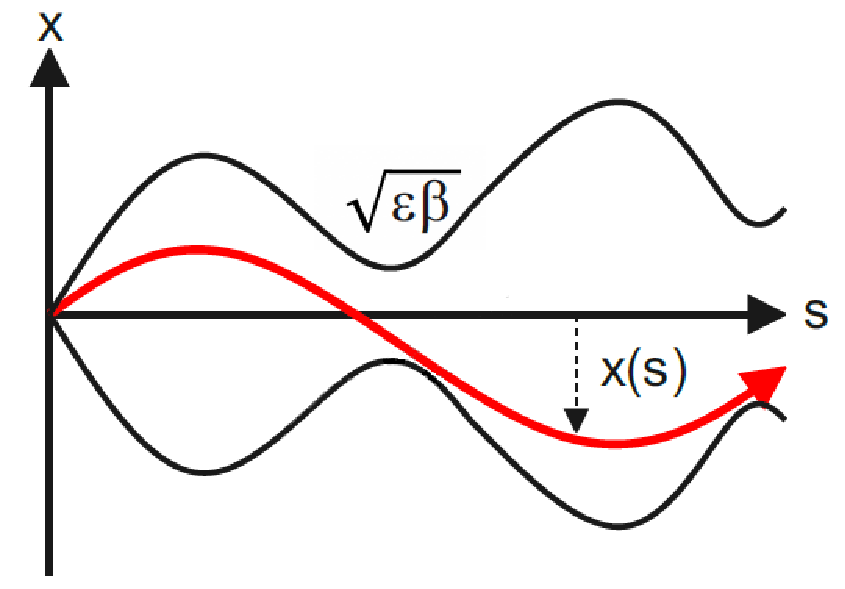
\includegraphics[width=0.6\textwidth]{Figures/Energy_Recovery_Linac_Design/Beam_Envelope_fixed.pdf}
\caption{Beam envelope (black) defined by a series of particle trajectories with size given by (Eq.~\ref{eq:envelope_function}). A possible single particle trajectory (red) in this beam of particles is highlighted.}
\label{fig:beam_envelope}
\end{figure}

The derivative of the trial solution (Eq.~\ref{eq:Hills_trial_solution}) shows the divergence of the particle trajectory with respect to $s$ and is given by
\begin{equation}
x'\left(s\right) = -\frac{\sqrt{\varepsilon}}{\sqrt{\beta\left(s\right)}}\left\{\alpha\left(s\right)\cos\left[\Psi\left(s\right)+\phi\right]+\sin\left[\Psi\left(s\right)+\phi\right]\right\}
\label{eq:Hills_trial_solution_derivative}    
\end{equation}
where the $\alpha\left(s\right)$ function, which relates to the orientation of the beam in phase space, is given by
\begin{equation}
\alpha\left(s\right) = -\frac{\beta'\left(s\right)}{2}.
\label{eq:alpha_function}    
\end{equation}
Taking the second derivative of the trial solution and substituting the trial solution (Eq.~\ref{eq:Hills_trial_solution}) and it's derivatives into Hill's equation (Eq.~\ref{eq:Hills_equation}) whilst understanding that the phase varies continually around the orbit and has a different value at each point on the trajectory \cite{wille2000physics}, the betatron phase can be calculated by
\begin{equation}
\Psi\left(s\right) = \int_{0}^{s}\frac{1}{\beta\left(s\right)}ds.
\label{eq:betatron_phase}    
\end{equation}

\subsection{Phase Space}

The phase space of a collection of particles represents the possible states of the dynamical system in a 6D representation, with each point in phase space illustrating a single particle \cite{jones2016design}. The 6D phase space is presented within the horizontal ($x$--$x'$), vertical ($y$--$y'$) and longitudinal ($z$--$z'$) planes. The phase space planes are position--divergence planes, in which the divergence of particle is closely related to it's momentum ($x' \propto p_{x}$). The solution to Hill's equation (Eq.~\ref{eq:Hills_trial_solution}) and it's derivative (Eq.~\ref{eq:Hills_trial_solution_derivative}) can be used to map the behaviour of a collection of particles within this phase space. 

Firstly, the trial solution and its derivative must be re-arranged to eliminate the betatron phase $\Psi\left(s\right)$ dependence. Re-arranging (Eq.~\ref{eq:Hills_trial_solution}) we obtain
\begin{equation}
\cos\left[\Psi\left(s\right)+\phi\right] = \frac{x\left(s\right)}{\sqrt{\epsilon\beta\left(s\right)}},
\label{eq:trial_phase_rearrangement}    
\end{equation}
which can be substituted into (Eq.~\ref{eq:Hills_trial_solution_derivative}) and re-arranged to yield
\begin{equation}
\sin\left[\Psi\left(s\right)+\phi\right] = \frac{\sqrt{\beta\left(s\right)}x'\left(s\right)}{\sqrt{\epsilon}} + \frac{\alpha\left(s\right)x\left(s\right)}{\sqrt{\varepsilon\beta\left(s\right)}}.
\label{eq:trial_derivative_phase_rearrangement}    
\end{equation}
Using the well-known trigonometric identity $\sin^{2}x+\cos^{2}x=1$, with (Eqs.~\ref{eq:trial_phase_rearrangement}, \ref{eq:trial_derivative_phase_rearrangement}) the phase space variables can be represented by
\begin{equation}
\frac{x\left(s\right)^{2}}{\beta\left(s\right)}+\left[\frac{\alpha\left(s\right)}{\sqrt{\beta\left(s\right)}}x\left(s\right)+\sqrt{\beta\left(s\right)}x'\left(s\right)\right]^{2} = \varepsilon,    
\label{eq:phase_space_trigonometry}
\end{equation}
which when expanded and then simplified, using the definition
\begin{equation}
\gamma\left(s\right) = \frac{1+\alpha\left(s\right)^{2}}{\beta\left(s\right)},
\label{eq:gamma_twiss}    
\end{equation}
relating to the angular size of the beam becomes
\begin{equation}
\varepsilon = \gamma\left(s\right)x\left(s\right)^{2}+2\alpha\left(s\right)x\left(s\right)x'\left(s\right)+\beta\left(s\right)x'\left(s\right)^{2},
\label{eq:phase_space_ellipse}    
\end{equation}
and $\varepsilon$ is defined as the single particle emittance or action. The form in (Eq.~\ref{eq:phase_space_ellipse}) is that of the equation of an ellipse; consequently the motion of a single particle around an orbit maps out an ellipse in phase space with area
\begin{equation}
A=\pi\varepsilon.
\label{eq:phase_space_area}    
\end{equation}
The parameters ($\beta\left(s\right)$, $\alpha\left(s\right)$, $\gamma\left(s\right)$) defined to interpret the phase space of a particle are collectively known as the Twiss parameters. Phase space ellipses are observed in each of the three planes as the results here are general. An example of the phase space ellipse in the $x$--$x'$ plane is shown in Fig.~\ref{fig:phase_space_diagram}.

\begin{figure}[!h]
\centering
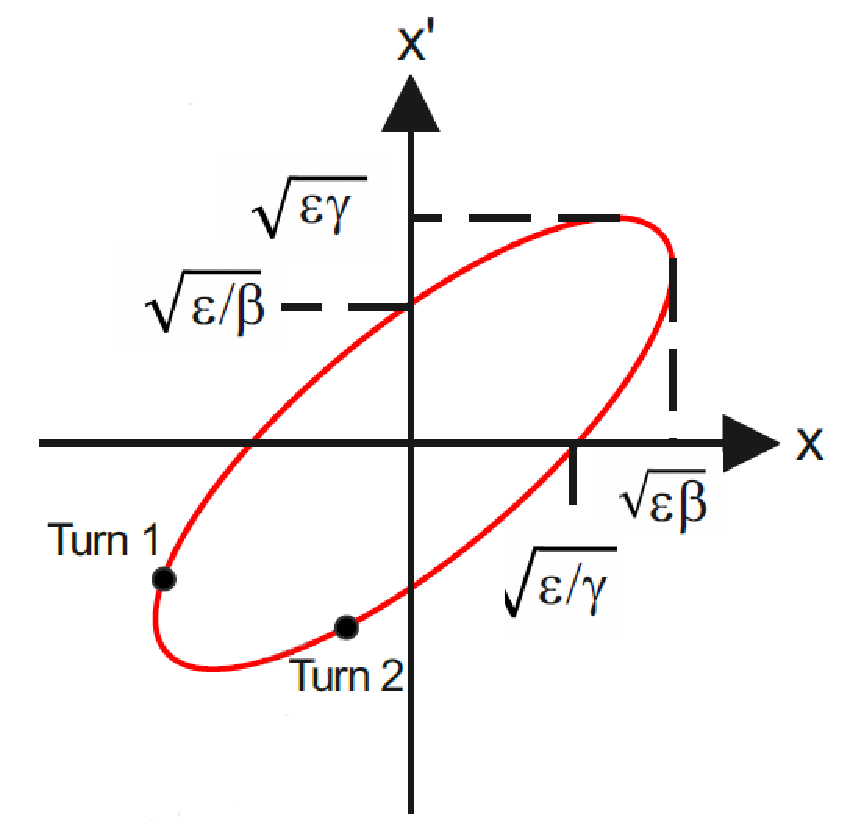
\includegraphics[width=0.6\textwidth]{Figures/Energy_Recovery_Linac_Design/phase_space_fixed.pdf}
\caption{Phase space ellipse (red) in horizontal $x$--$x'$ phase space. Dimensions of the phase space ellipse are highlighted, the tilt of the ellipse relates to the $\alpha$ parameter. Particles traverse within the phase space ellipse with phase advance $\mu$ with area $\pi\varepsilon$.}
\label{fig:phase_space_diagram}
\end{figure}


Since the phase space ellipse is for a single particle trajectory, the emittance is the single particle emittance. This is unsatisfactory for describing an ensemble of particles, therefore the concept of emittance requires extension to a many-particle ensemble -- the \textit{rms} emittance of a particle beam. To extend the single particle emittance $\varepsilon$ to the \textit{rms} emittance $\epsilon$, the \textit{rms} emittance must be of the form
\begin{equation}
\epsilon_{rms} = \sqrt{\frac{1}{m}\sum_{i}^{i=m}\varepsilon_{i}} = \sqrt{\frac{1}{m}\left(\varepsilon_{1}+\varepsilon_{2}+\ldots+\varepsilon_{m}\right)},
\label{eq:rms_emittance_transform}    
\end{equation}
where $m$ is the no. particles. The \textit{rms} emittance $\epsilon$ is an average of the single particle emittances of the bunch with the typical \textit{rms} transform and consequently can be re-cast, by inspection of (Eq.~\ref{eq:phase_space_ellipse}), as a function of the average position and divergence of the particles
\begin{equation}
\epsilon = \sqrt{\langle x^{2}\rangle\langle x'^{2}\rangle-\langle xx'\rangle^{2}},
\label{eq:rms_emittance}    
\end{equation}
where the average position $\langle x\rangle$ and divergence $\langle x'\rangle$ terms can be expressed in terms of the Twiss parameters
\begin{align}
\langle x^{2}\rangle &= \beta_{x}\epsilon_{x}, \nonumber\\
\langle x'^{2}\rangle &= \gamma_{x}\epsilon_{x}, \nonumber\\
\langle xx'\rangle &= -\alpha_{x}\epsilon_{x}.
\label{eq:rms_emittance_twiss}    
\end{align}
Whilst the discussion here is for the $x$ (horizontal) plane, the description is analagous in the $y$ (vertical) plane. The \textit{rms} horizontal spot size of the particle beam becomes
\begin{equation}
\sigma_{x} = \sqrt{\beta_{x}\epsilon_{x}},
\label{eq:spot_size_particle}    
\end{equation}
following the description of the envelope function (Eq.~\ref{eq:envelope_function}).

Liouville's theorem \cite{liouville1838note}, as commonly applied in statistical mechanics \cite{gibbs1902elementary}, maintains that the phase-space density of a system remains unchanged under conservative forces applied to the system. Applied to the accelerator situation of harmonic oscillation around a reference orbit due to conserved magnetic forces, Liouville's theorem implies that the emittance is conserved throughout the beamline unless the beam of particles is acted upon by a non-conservative force. Therefore, under conservative forces, the propagation of Twiss parameters can be accomplished similarly to the transform of phase space co-ordinates. For example, in the horizontal plane phase space co-ordinates can be transformed from an initial state ($x_{0}$, $x'_{0}$) to a final state ($x_{1}$, $x'_{1}$) via transport matrices such that
\begin{equation}
\begin{pmatrix}
x_{1} \\
x'_{1}
\end{pmatrix}
=
\begin{pmatrix}
\boldsymbol{R}_{11} & \boldsymbol{R}_{12} \\
\boldsymbol{R}_{21} & \boldsymbol{R}_{22}
\end{pmatrix}
\begin{pmatrix}
x_{0} \\
x'_{0}
\end{pmatrix}.
\label{eq:general_phase_space_transform}
\end{equation}
Expanding the matrices in (Eq.~\ref{eq:general_phase_space_transform}) and re-casting the equations for substitution into (Eq.~\ref{eq:phase_space_ellipse}), the analagous transform of the Twiss parameters from initial state ($\beta_{0}$, $\alpha_{0}$, $\gamma_{0}$) to final state ($\beta_{1}$, $\alpha_{1}$, $\gamma_{1}$) becomes 
\begin{equation}
\begin{pmatrix}
\beta_{1} \\
\alpha_{1} \\
\gamma_{1} 
\end{pmatrix}
=
\begin{pmatrix}
\boldsymbol{R}_{11}^{2} & -2\boldsymbol{R}_{11}\boldsymbol{R}_{12} & \boldsymbol{R}_{12}^{2} \\
-\boldsymbol{R}_{11}\boldsymbol{R}_{21} & \boldsymbol{R}_{12}\boldsymbol{R_{21}}+\boldsymbol{R}_{11}\boldsymbol{R}_{22} & -\boldsymbol{R}_{12}\boldsymbol{R}_{22} \\
\boldsymbol{R}_{21}^{2} & -2\boldsymbol{R}_{21}\boldsymbol{R}_{22} & \boldsymbol{R}_{22}^{2} 
\end{pmatrix}
\begin{pmatrix}
\beta_{0} \\
\alpha_{0} \\
\gamma_{0}
\end{pmatrix}.
\label{eq:general_Twiss_transform}
\end{equation}

\subsection{Periodic Lattices and Stability}

A periodic lattice, for example a repeating series of beamline elements, named cells, with length $L_{\mathrm{cell}}$, which adheres to the property $\boldsymbol{R}\left(s\right) = \boldsymbol{R}\left(s+L_{\mathrm{cell}}\right)$, where the Twiss parameters are unchanged ($\beta_{0}=\beta_{1}=\beta$, $\alpha_{0}=\alpha_{1}=\alpha$, $\gamma_{0}=\gamma_{1}=\gamma$). Therefore, a periodic cell has the single plane transport matrix of the form
\begin{equation}
\boldsymbol{R} =
\begin{pmatrix}
\cos\mu + \alpha\sin\mu & \beta\sin\mu \\
-\gamma\sin\mu & \cos\mu-\alpha\sin\mu
\end{pmatrix}
\label{eq:periodic_transport_matrix}    
\end{equation}
where $\mu$ is the phase advance per cell. The Twiss parameters of the periodic lattice can be related to the transport matrix via re-arrangement of the periodic transport matrix (Eq.~\ref{eq:periodic_transport_matrix})
\begin{align}
\beta &= \frac{\boldsymbol{R}_{12}}{\sin\mu}, 
\label{eq:periodic_beta_function} \\
\alpha & = \frac{\boldsymbol{R}_{11}-\boldsymbol{R}_{22}}{2\sin\mu},
\label{eq:periodic_alpha} \\
\gamma &= \frac{1+\left(\boldsymbol{R}_{11}-\boldsymbol{R}_{22}\right)^{2}}{4\boldsymbol{R}_{12}\sin\mu},
\label{eq:periodic_gamma} \\
\mu &= \cos^{-1}\left(\frac{\boldsymbol{R}_{11}-\boldsymbol{R}_{22}}{2}\right),
\label{eq:periodic_phase_advance}
\end{align}
and the periodic $\gamma$ function is defined by (Eq.~\ref{eq:gamma_twiss}).

The periodic focusing system within an accelerator is stable if the eigenvectors of the transport matrix remain real for many passes through the accelerator beamline because the phase of the particles remains real. Therefore, the eigenvectors of the transport matrix can be found through the equation
\begin{equation}
\left(\boldsymbol{R}-\lambda\boldsymbol{I}\right)\boldsymbol{X} = 0,
\label{eq:eigenvalues_equation}    
\end{equation}
where $\boldsymbol{R}$ is the transport matrix, $\lambda$ are the eigenvalues of the system, $\boldsymbol{I}$ is the identity matrix and $\boldsymbol{X}$ is a vector of the relevant phase space variables. It follows from the periodic transport matrix that the sum of the eigenvalues of $\boldsymbol{R}$ must satisfy
\begin{equation}
\sum\lambda = \boldsymbol{\mathrm{Tr}}\left(\boldsymbol{R}\right) = 2\cos\mu,
\label{eq:eigenvalue_stability}
\end{equation}
where $\boldsymbol{\mathrm{Tr}}\left(\boldsymbol{R}\right)$ is the trace of the transport matrix. As previously mentioned, the trace of the transport matrix must satisfy (Eq.~\ref{eq:eigenvalues_equation}) for many passes through the accelerator beamline, which for a periodic lattice is typically constructed from many periodic cells. Consequently the stability criterion is expanded to become
\begin{equation}
\boldsymbol{\mathrm{Tr}}\left(\boldsymbol{R}^{N}\right) = 2\cos\left(N\mu\right) \leq 2, 
\label{eq:stability_criterion}    
\end{equation}
where $N$ is the number of periodic cells traversed.

\subsection{Dispersion and Off-Momenta Particles} 
\label{sec:dispersion_off_momentum_particles}

Dispersion is defined as the variation in position of a particle due to the variation in its momentum from the design momentum, as introduced in Section~\ref{sec:equations_of_motion}. Particles that vary from the design momentum vary from typical betatron motion $\boldsymbol{X}_{\beta}$, with an additional dispersive motion term $\boldsymbol{X}_{\Delta p/p_{0}}$ i.e $\boldsymbol{X} = \boldsymbol{X}_{\beta} + \boldsymbol{X}_{\Delta p/p_{0}}$. Therefore, the matrix representation of the propagation of dispersive particles becomes
\begin{equation}
\boldsymbol{X}_{1} = \boldsymbol{R}\boldsymbol{X}_{\beta} + \boldsymbol{R}\boldsymbol{X}_{\Delta p/p_{0}},
\label{eq:dispersive_transport_matrix_propagation}    
\end{equation}
which, taking the $x$--$x'$ plane as an example, can be accounted for using a transform including the dispersive motion
\begin{equation}
\begin{pmatrix}
x_{1} \\
x'_{1} \\
\Delta p /p_{0}
\end{pmatrix}
=
\begin{pmatrix}
\boldsymbol{R}_{1,1} & \boldsymbol{R}_{1,2} & \boldsymbol{R}_{1,6} \\
\boldsymbol{R}_{2,1} & \boldsymbol{R}_{2,2} & \boldsymbold{R}_{2,6} \\
0 & 0 & 1
\end{pmatrix}
\begin{pmatrix}
x_{0} \\
x'_{0} \\
\Delta p / p_{0} 
\end{pmatrix}
\label{eq:dispersive_transport_simplified}
\end{equation}
where the index 6 is used as this is the column of a 6D transport matrix that would include these dispersive terms. A dispersion function $\eta\left(s\right)$ can be defined for the motion of the particle by neglecting the betatron motion and setting $\Delta p/p_{0} =1$
\begin{equation}
\begin{pmatrix}
\eta_{x}\left(s\right) \\
\eta'_{x}\left(s\right) \\
1
\end{pmatrix}
=\boldsymbol{R}
\begin{pmatrix}
x_{0} \\
x'_{0} \\
1
\end{pmatrix}.
\label{eq:dispersion_function}    
\end{equation}
The periodic dispersion ($\eta_{x}\left(s\right)=\eta_{x}$, $\eta'_{x}\left(s\right)=\eta'_{x}$) can be found via re-arrangement of (Eq.~\ref{eq:dispersion_function}) using the transport matrix in (Eq.~\ref{eq:dispersive_transport_simplified}) in terms of the transport matrix elements
\begin{align}
\eta_{x} &= \frac{\boldsymbol{R}_{13}\left(1-\boldsymbol{R}_{22}\right)+\boldsymbol{R}_{12}\boldsymbol{R}_{23}}{\left(1-\boldsymbol{R}_{11}\right)\left(1-\boldsymbol{R}_{22}\right)-\boldsymbol{R}_{21}\boldsymbol{R}_{12}},
\label{eq:periodic_dispersion} \\
\eta'_{x} &= \frac{\boldsymbol{R}_{23}\left(1-\boldsymbol{R}_{11}\right)+\boldsymbol{R}_{21}\boldsymbol{R}_{13}}{\left(1-\boldsymbol{R}_{11}\right)\left(1-\boldsymbol{R}_{22}\right)-\boldsymbol{R}_{21}\boldsymbol{R}_{12}}.
\label{eq:periodic_dispersion_prime}
\end{align}

The beam size of a dispersive particle beam (for a periodic lattice) can be defined, baring similarity to (Eq.~\ref{eq:dispersive_transport_matrix_propagation}), through an extension of the beam size due to betatron motion (Eq.~\ref{eq:horizontal_emittance})
\begin{equation}
\sigma_{x} = \sqrt{\epsilon_{x}\beta_{x}} + \eta_{x}\frac{\Delta p}{p_{0}}.
\label{eq:dispersive_beam_size}    
\end{equation}
An extension to the definition of the phase space ellipse (Eq.~\ref{eq:phase_space_ellipse}) is also possible for the case of a dispersive beam where the phase space plane variables ($x$--$x'$ etc.) can be replaced by the dispersion functions
\begin{equation}
\mathcal{H} = \beta\eta'^{2}+2\alpha\eta\eta'+\gamma\eta^{2},
\label{eq:dispersive_phase_space_ellipse}    
\end{equation}
where $\mathcal{H}$ is analogous to the emittance in defining the area of the phase space ellipse for a dispersive beam.

\section{Tune and Chromaticity}

\subsection{Tune}

The tune of an accelerator is defined as the number of betatron oscillations per revolution around the circumference of a re-circulated accelerator
\begin{equation}
Q=\frac{N\mu}{2\pi} = \frac{1}{2\pi}\oint\frac{1}{\beta}ds,
\label{eq:accelerator_tune}    
\end{equation}
where $N$ is the no. periodic cells within the accelerator, and the integral $\oint$ relates to an integral around the circumference of the accelerator. However, often accelerator beamlines aren't entirely periodic. For example, areas of the beamline can be devoted to focusing to a small spot size for a collider and inverse Compton scattering source or be subject to insertion devices such as undulator magnets. Therefore, it is often more useful to define the tune per cell of a section of the beamline with length $L_{\mathrm{cell}}$
\begin{equation}
Q=\frac{\mu}{2\pi} = \frac{1}{2\pi}\int_{0}^{L_{\mathrm{cell}}}\frac{1}{\beta}ds. 
\label{eq:tune_per_cell}    
\end{equation}

In re-circulated accelerators such as storage rings, the particle beam is subject to the same collection of magnetic elements many times. For example, in the MAX-III storage ring the beam lifetime at 250~\si{\milli\ampere} is 11.3~\si{\hour} with a 36~\si{\meter} circumference (120~\si{\nano\second} revolution time) resulting in $\sim3.4\times 10^{11}$ revolutions per bunch. Therefore, the beam is acted upon by periodic transverse forces causing transverse oscillations of the beam which, under certain conditions, may result in the circulating beam resonating \cite{wille2000physics}. A transversely resonating beam oscillation -- known as an optical resonance -- could cause large beam amplitudes which would result in beam sizes that could not be contained within the beampipe and the particles would be lost.

A full discussion and derivation of the conditions required for optical resonances is beyond the scope of this thesis, instead for brevity the discussion by K. Willie \cite{wille2000physics} is recommended and we utilise the result for the relationship between expected optical resonance behaviour and tune
\begin{equation}
mQ_{x}+nQ_{y} = p,
\label{eq:tune_resonances}    
\end{equation}
where $m$, $n$ and $p$ are integers. Resonances in accelerators occur at integer and fractional-integer tunes ($p = n + 1/3, 1/2, 1, 2$ etc.) and can be coupled resonances, hence why the tunes in both transverse planes are included in (Eq.~\ref{eq:tune_resonance}). The order of the resonance is found via $\left|m\right| + \left|n\right|$, and the strength of the resonance decreases rapidly as a function of order. Consequently, the tunes in an accelerator must be chosen to avoid optical resonances, which is fundamental at the design stage and is often named the working point. The working point is often displayed in a $Q_{x}$--$Q_{y}$ tune diagram, as shown in Fig.~\ref{fig:tune_diagram}, where the resonances up to $n$th order are typically displayed.  

\begin{figure}[!h]
\centering
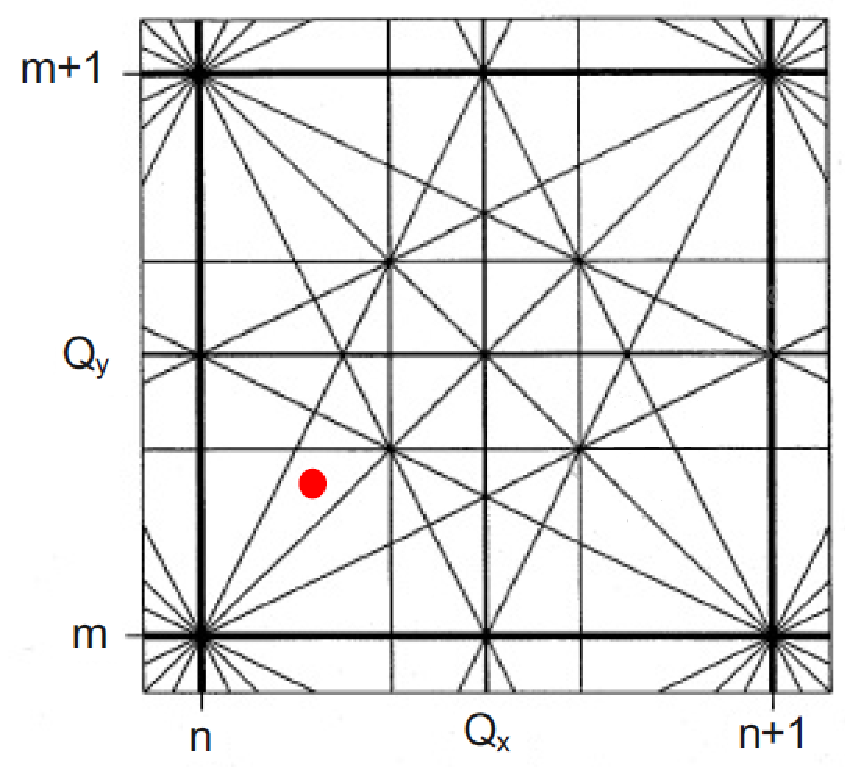
\includegraphics[width=0.6\textwidth]{Figures/Energy_Recovery_Linac_Design/Tune_Diagram_fixed.pdf}
\caption{Tune diagram up to 3rd order showing possible locations of optical resonances \cite{wille2000physics} (black). A possible working point (red) is located away from lines of optical resonance.}
\label{fig:tune_diagram}
\end{figure}

\subsection{Chromaticity}

Chromaticity is defined as the variation in tune due to the variation in momentum within an accelerator as given by
\begin{equation}
\xi = \frac{\Delta Q}{\Delta p/p_{0}},
\label{eq:accelerator_chromaticity}    
\end{equation}
where the variation in tune is driven by the chromatic aberration focusing errors that occur when off-momentum particles traverse focusing magnets, as presented for a quadrupole in Fig.~\ref{fig:chromatic_aberration}.

\begin{figure}[!h]
\centering
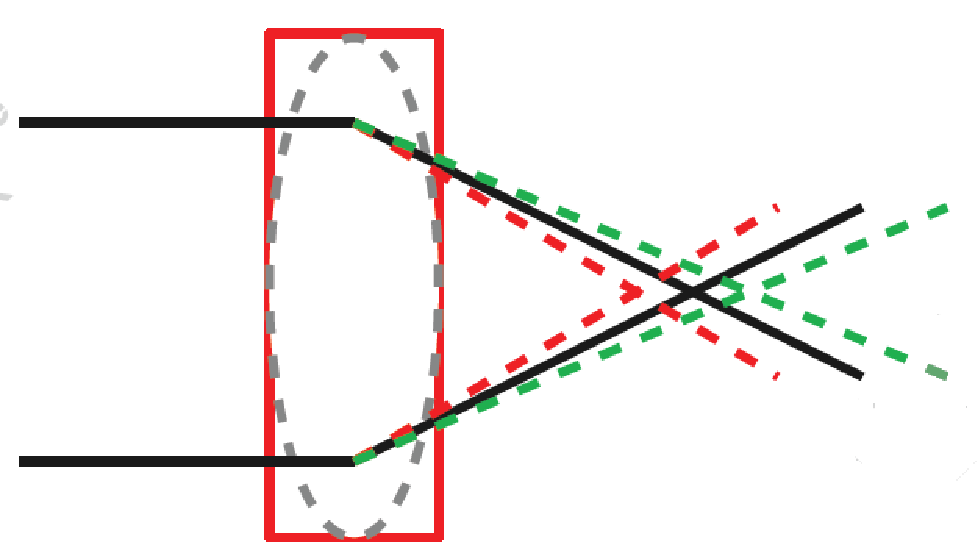
\includegraphics[width=0.6\textwidth]{Figures/Energy_Recovery_Linac_Design/Chromatic_Aberration_fixed.pdf}
\caption{Particle trajectories of a reference particle (black), a particle with higher energy ($\Delta p/p_{0}>0$) (green, dashed) and a particle with lower energy ($\Delta p/p_{0}<0$) through a focusing quadrupole (red). Focal lengths are increased for particles with higher energy and decreased for lower energy particles, hence a chromatic aberration occurs. }
\label{fig:chromatic_aberration}
\end{figure}

The chromatic effect of a quadrupole magnet can there for be considered as
\begin{align}
\xi_{x} &= -\frac{1}{4\pi}\int\beta_{x}k_{1}ds, \\
\xi_{y} &= \frac{1}{4\pi}\int\beta_{y}k_{1}ds.
\label{eq:quadrupole_chromaticity}
\end{align}
where it is noted that for periodic focusing the $\beta_{x}$-function is typically larger upon entrance to the focusing quadrupole and the $\beta_{y}$ function is larger in the defocusing quadrupole, therefore the natural chromaticity throughout a periodic focusing accelerator is negative. 

Correction of chromaticity is typically conducted by sextupole ($n=3$) magnets with fields described by (Eq.~\ref{eq:sextupole_magnetic_field}),with focusing dependent on transverse beam position. Sextupoles are placed in dispersive sections of the accelerator where the transverse position of the particles is dependent upon the momentum of the particle so the transverse field dependence can be used to correct the aberrations. 

\section{Longitudinal Dynamics and RF Acceleration}

Previous discussions within this section have been focused on the transverse motion of particles throughout the accelerator beamline. However a similar analysis can also be applied to the longitudinal dimension where, instead of magnetic bending and focusing fields, electric fields used in the acceleration of particles dominate the dynamics. Analysis of longitudinal dynamics focuses on the energy of the particles, their longitudinal position relative to the centroid of the ensemble as well as the stability and phase of the longitudinal motion. This section focuses on the effect of bending and dispersive motion upon the longitudinal dynamics, then upon investigation of the longitudinal equations of motion and phase space and finally the effect of magnetic elements upon the longitudinal dimensions of the beam is explored.

\subsection{Momentum Compaction}
\label{sec:momentum_compaction}

The path length $L$ of a particle trajectory as a function of momentum variation can be wrote as a Maclaurin series \cite{wolski2012longitudinal}
\begin{equation}
L = L_{0}\left[1+\alpha_{p}\frac{\Delta p}{p_{0}}+\frac{1}{2}\alpha_{p}^{\left(2\right)}\left(\frac{\Delta p}{p_{0}}\right)^{2}\right],
\label{eq:path_length_expansion}    
\end{equation}
where $L_{0}$ is the path length of the reference particle ($\Delta p/p_{0}=0$). Whilst higher order momentum compaction terms are present in the expansion (Eq.~), such as $\alpha_{p}^{\left(2\right)}$, to first order this can be simplified to
\begin{equation}
\alpha_{p} = \frac{1}{L}\frac{dL}{\Delta p/p_{0}},
\label{eq:momentum_compaction_first_order}    
\end{equation}
where $\alpha_{p}$ is the linear momentum compaction. Consider the trajectory of a particle through a curved reference trajectory -- subject to a dipole bending field -- moving with a displacement $x$ from the reference trajectory, the path length of this element is given by
\begin{equation}
dL = \left(\rho+x\right)d\theta = \left(1+\frac{x}{\rho}\right)ds.
\label{eq:displaced_bend_trajectory}    
\end{equation}
The total path length of the displaced trajectory through the bending field is given by the integral of (Eq.~\ref{eq:displaced_bend_trajectory})
\begin{equation}
L = \int_{0}^{L_{0}} 1+\frac{x}{\rho} ds = L_{0} + \int_{0}^{L_{0}}\frac{x}{\rho}ds, 
\label{eq:displaced_bend_path_length}    
\end{equation}
If we consider the displacement in $x$ to arise purely because of dispersive motion, then $x$ becomes
\begin{equation}
x = \eta_{x}\frac{\Delta p}{p} + \frac{1}{2}\eta_{x}^{\left(2\right)}\left(\frac{\Delta p}{p}\right)^{2},
\label{eq:dispersive_displacement}    
\end{equation}
where the higher order dispersion terms $\eta_{x}^{\left(2\right)}$ are neglected. The displacement due to dispersive motion (Eq.~\ref{eq:dispersive_displacement}) is substituted into the path length of the curved trajectory (Eq.~\ref{eq:displaced_bend_path_length}) yielding
\begin{align}
L &= L_{0} + \frac{\Delta p}{p_{0}}\int_{0}^{L_{0}}\frac{\eta_{x}}{\rho}ds, &
\Delta L &= \frac{\Delta p}{p_{0}}\int_{0}^{L_{0}}\frac{\eta_{s}}{\rho}ds,
\label{eq:dispersive_path_length_variation}
\end{align}
which via substitution into (Eq.~\ref{eq:momentum_compaction_first_order}) and re-arrangement yields the momentum compaction in terms of dispersion
\begin{equation}
\alpha_{p} = \frac{1}{L_{0}}\int_{0}^{L_{0}}\frac{\eta_{x}}{\rho}ds.
\label{eq:momentum_compaction_dispersion}    
\end{equation}

Inspection of (Eq.~\ref{eq:momentum_compaction_dispersion}), demonstrates that momentum compaction only arises in dispersive sections where the reference trajectory is curved, such as in dipoles, because in straight sections $\rho\rightarrow\infty$ and therefore the contribution of these terms are negligible. 

\subsection{RF Acceleration}
\label{sec:RF_acceleration}

A particle, or collection of particles, can be accelerated by an electric field $\overrightarrow{E}$ satisfying the wave equation, displayed here in vacuum
\begin{equation}
\nabla^{2}\overrightarrow{E}-\frac{1}{c^{2}}\frac{\partial^{2}\overrightarrow{E}}{\partial t^{2}},
\label{eq:electromagnetic_wave_equation}    
\end{equation}
which (in our local co-ordinate system) is applied in the longitudinal direction. Most modern accelerators use powerful radio-frequency systems, or RF cavities, to produce the requisite strong electric fields, with frequencies from \si{\kilo\hertz} to \si{\giga\hertz} \cite{wille2000physics}, required to accelerate the particles to energies on the \si{\mega\electronvolt} to \si{\tera\electronvolt} scale. Whilst other acceleration methods exist such as electrostatic acceleration \cite{bromley1974development}, dielectric wakefield acceleration \cite{mtingwa1990theory} and laser plasma wakefield acceleration \cite{sprangle1988laser,esarey2009physics}, we limit our discussion to RF acceleration.

The solution to (Eq.~\ref{eq:electromagnetic_wave_equation}) for an RF cavity, where the local ($x$, $y$, $z$) co-ordinate system is used, is of the form
\begin{equation}
\overrightarrow{E}\left(z,t\right) = E_{0}\exp\left[i\left(kz-\omega t\right)\right],
\label{eq:RF_cavity_electric_field}    
\end{equation}
where the phase of the electric field is encapsulated by the synchronous phase $\psi = kz-\omega t$. The energy gain of a particle in an electric field, re-cast in terms of the phase, is given by 
\begin{equation}
\Delta E = e \int E_{0}\exp\left(i\psi\right)dz = eV\left(\psi\right),
\label{eq:particle_energy_gain_RF}    
\end{equation}
where $V\left(\psi\right)$ is the RF voltage as a function of phase. Therefore, to maintain a constant energy gain within all subsequent RF cavities, the phase must remain constant at the RF cavity
\begin{equation}
\frac{d\psi}{dt} = k\beta c-\omega = 0. 
\label{eq:synchronicity_condition}   
\end{equation}
Consequently, the transit time between RF cavities and revolution frequency of the particle must remain constant for subsequent acceleration at identical phase. For an accelerator of path length $L$, the solution is of the form $k=2\pi/L$ where $\omega=\omega_{\mathrm{rev}}$ is the revolution frequency. The RF frequency can operate at any integer value of this revolution frequency, named the harmonic number $h$, and still satisfy the synchronicity condition (Eq.~\ref{eq:synchronicity_condition}), therefore the wavenumber and frequency of the accelerating RF waveform have the form
\begin{align}
k_{h} = \frac{2\pi h}{L_{0}},
\label{eq:RF_wavenumber} \\
f_{RF} = \frac{h\omega_{\mathrm{rev}}}{2\pi}.
\label{eq:RF_frequency}
\end{align}

The transit time $T$ between RF cavities is affected by off-momenta particles, similarly to the path length in momentum compaction studies (see Section~\ref{sec:momentum_compaction}), therefore the transit time with respect to the reference particle ($\Delta p/p_{0}$=0) can be expanded via a Maclaurin series to account for the momentum variation
\begin{equation}
T = T_{0}\left[1+\eta_{p}\frac{\Delta p}{p_{0}}+\frac{1}{2}\eta_{p}^{\left(2\right)}\left(\frac{\Delta p}{p_{0}}\right)^{2}\right],
\label{eq:transit_time_expansion}    
\end{equation}
where $\eta_{p}$ is named the phase slip factor. Neglecting non-linear terms and re-arranging (Eq.~\ref{eq:transit_time_expansion}) becomes
\begin{equation}
\eta_{p} = \frac{\Delta T/T}{\Delta p/p_{}0},
\label{eq:phase_slip_factor_transit_time}    
\end{equation}
where the transit time is a function of path length $L$, $T = L/\beta c$, which can be used to re-cast the phase slip factor (Eq.~\ref{eq:phase_slip_factor_transit_times}) as  
\begin{equation}
\eta_{p} = \frac{\Delta T/T}{\Delta p/p} = \frac{\Delta L/L_{0}}{\Delta p/p_{0}}-\frac{\Delta\beta/\beta}{\Delta p/p_{0}}.
\label{eq:phase_slip_factor_expansion}    
\end{equation}
The Lorentz speed factor term in (Eq.~\ref{eq:phase_slip_factor_expansion}) can be related to the Lorentz factor \cite{wolski2012longitudinal} by 
\begin{equation}
\frac{\Delta\beta/\beta}{\Delta p/p_{0}} = \frac{1}{\gamma^{2}},
\label{eq:phase_slip_Lorentz_relation}    
\end{equation}
therefore using the definition of the momentum compaction factor (Eq.~\ref{eq:momentum_compaction_first_order}) and the relationship for the Lorentz speed factor term (Eq.~\ref{eq:phase_slip_factor_expansion}), the phase slip factor becomes
\begin{equation}
\eta_{p} = \alpha_{p} - \frac{1}{\gamma^{2}}.
\label{eq:phase_slip_factor}    
\end{equation}

Three distinct regimes exist within the longitudinal dynamics relating to the phase slip factor (Eq.~\ref{eq:phase_slip_factor}), relating to the transition between relativistic motion:
\begin{itemize}
    \item{Below transition ($\eta_{p}<0$), where $\alpha_{p}<0 \parallel \alpha_{p}<1/\gamma^{2}$ and the synchronous phase is $0<\psi<\pi/2$.
    \begin{itemize}
        \item{The revolution frequency increases with increasing energy.}
        \item{Higher energy particles arrive at the RF cavity first due to their higher velocity.}
    \end{itemize}}
    \item{At transition ($\eta_{p}=0$), where $\alpha_{p}=1/\gamma^{2}$.
    \begin{itemize}
        \item{The revolution frequency is independent of energy.} 
    \end{itemize}}
    \item{Above transition ($\eta_{p}>0$), where $\alpha_{p}>1/\gamma^{2}$ and the synchronous phase is $\pi/2<\psi<\pi$.
    \begin{itemize}
        \item{The revolution frequency decreases with increasing energy.}
        \item{Higher energy particles arrive at the the RF cavity last because they traverse a longer path and their higher velocity is of no advantage since $\beta\approx1$.}
    \end{itemize}}
\end{itemize}
The longitudinal dynamics above transition are shown in Fig.~\ref{fig:phase_focusing_above_transition}. At first glance, the reason for the mandated synchronous phases above and below transition is unclear however, this is to take advantage of longitudinal phase focusing. 

\begin{figure}[!h]
\centering
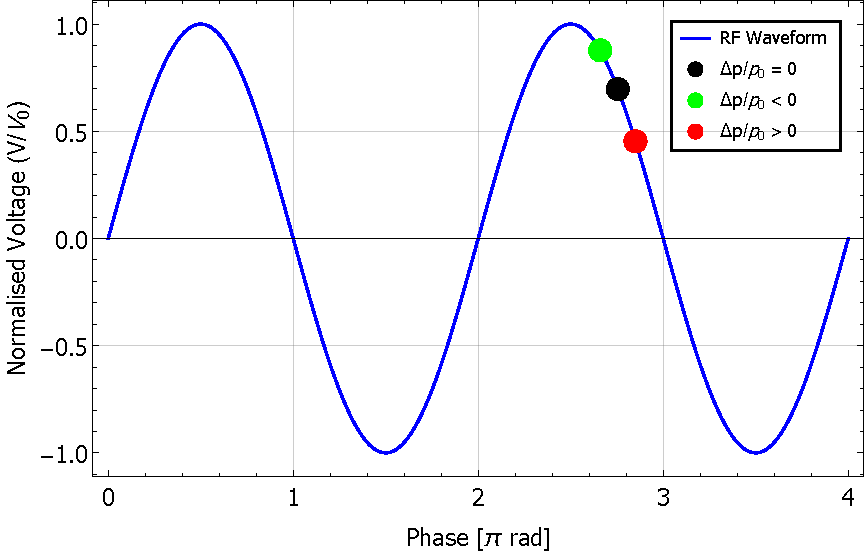
\includegraphics[width=0.7\textwidth]{Figures/Energy_Recovery_Linac_Design/Above_Transition_Phase_Focusing.pdf}
\caption{Schematic of off-crest acceleration providing longitudinal phase focusing. The normalised RF voltage of an RF cavity is shown as a function of synchronous phase. A reference particle (black, $\Deltap/p_{0}=0$) is accelerated off-crest, where the early particle (green, $\Delta p/p_{0}<0$) is accelerated by a higher voltage and the late particle (red, $\Delta p/p_{0}>0$) is accelerated to by a lesser voltage. Greater acceleration (energy gain) increases path length, increasing the transit time. }
\label{fig:phase_focusing_above_transition}
\end{figure}

Longitudinal phase focusing takes advantage of the sinusoidal nature of the accelerating electric field (Eq.~\ref{eq:RF_cavity_electric_field}) to bias the acceleration of off-momenta particles, with varying transit times, to restore their phase toward the synchronous phase. The longitudinal phase focusing technique is shown in Fig.~\ref{fig:phase_focusing_above_transition}. Above transition, a particle with reduced momentum ($\Delta p/p_{0}<0$) will arrive at the RF cavity earlier, and receiving a larger energy gain will increase its transit time  as its path length will increase. However, a particle that arrives late ($\Delta p/p_{0}>0$) will receive a smaller energy gain and therefore traverse a shorter path length, arriving earlier next revolution.
The voltage, and therefore the energy gain, vary sinusoidally as a function of phase where maximum energy gain is at $\psi=\pi/2$ -- the crest of the electromagnetic wave in the RF cavity. However, setting the synchronous phase to an off-crest position in the range $\pi/2<\psi<\pi$, the slope of the RF voltage around this point is near-linear which is appropriate to achieve the varying energy gain required for longitudinal phase focusing.  

Following the example of Jones \cite{jones2016design}, if the variation in energy and other related beam parameters within a recirculated accelerator is small with relation to phase then the longitudinal equation of motion is of the form 
\begin{equation}
\frac{d^{2}\psi}{dt^{2}} + \beta ck_{h}\eta_{p}\frac{\partial}{\partial t}\left(c\frac{\Delta p}{p_{0}}\right) = 0,
\label{eq:longitudinal_equation_of_motion}
\end{equation}
which can be simplified by assuming a linear expansion of the synchronous phase, and expressed in terms of either the phase or the momentum deviation
\begin{align}
\frac{d^{2}\psi}{dt^{2}} + \Omega^{2}\psi = 0,
\label{eq:longitudinal_equation_of_motion_phase} \\
\frac{d^{2}\left(\Delta p/p_{0}\right)}{dt^{2}} + \Omega^{2}\frac{\Delta p}{p_{0}} = 0,
\label{eq:longitudinal_equation_of_motion_momentum}
\end{align}
where the synchronous phase and momentum are related via
\begin{equation}
\frac{\Delta p}{p_{0}} = -\frac{1}{h\omega_{\mathrm{RF}}\eta_{p}}\frac{d\psi}{dt},
\label{eq:momentum_synchronous_phase_relation}    
\end{equation}
and assuming the RF frequency is a harmonic of the revolution frequency $\omega_{\mathrm{rev}}=2\pi f_{\mathrm{RF}}/h$ and that the RF cavity produces a sinusoidal RF wave $V=V_{0}\sin\psi$, with RF voltage $V$, the synchrotron oscillation frequency is given by
\begin{equation}
\Omega^{2} = \frac{\omega_{\mathrm{rev}}^{2}h\eta_{p}eV_{0}\cos\psi}{2\pi\beta cp_{0}}.
\label{eq:synchrotron_oscillation_frequency}    
\end{equation}
Synchrotron oscillations in the longitudinal plane typically have a lower frequency than the aforementioned betatron oscillations in the transverse planes. The equation of motion in the longitudinal plane (Eq.~\ref{eq:longitudinal_equation_of_motion_phase}) produces a stable $\psi$--$\Delta p/p$ phase space ellipse when motion is damped ($\Omega^{2}>0$) and is described by a hyperbola in phase space when motion is unstable and anti-damped ($\Omega^{2}<0$). The equation of motion therefore generates a series of ellipses separated by regions of unstable hyperbolic regions which form separatrixes in phase space, as displayed in Fig.~\ref{fig:longitudinal_dynamics}.

\begin{figure}[!h]
\centering
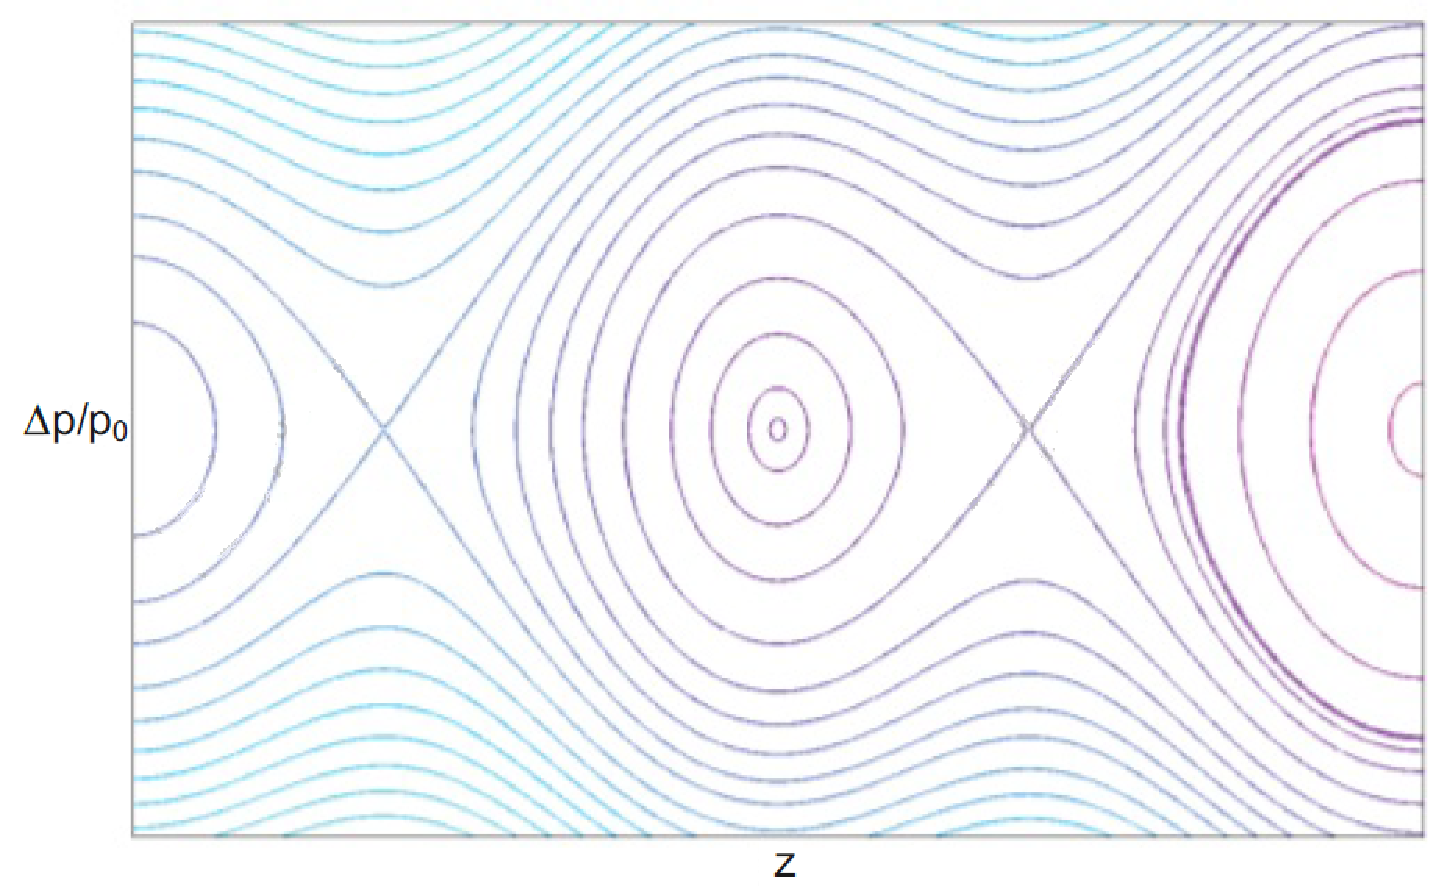
\includegraphics[width=0.7\textwidth]{Figures/Energy_Recovery_Linac_Design/Longitudinal_Dynamics_fixed.pdf}
\caption{Longitudinal phase space diagram, with the fractional variation in momentum as a function of longitudinal displacement. Closed ellipses represent stable regions ($\Omega^{2}>0$) of longitudinal phase space whereas hyperbolic regions represent unstable ($\Omega^{2}<0$) particle trajectories. Separatrixes show the limits of an RF bucket. Reproduction of longitudinal phase space diagram by A. Wolski \cite{wolski2012longitudinal}.}
\label{fig:longitudinal_dynamics}
\end{figure}

The region of stable motion within the separatrix is named the RF bucket, and particles within an RF bucket form a bunch with bunch length proportional to the size of the RF bucket transformed to the longitudinal position. Bunches are sub-divisions of accelerator beams. The maximum momentum deviation of an RF bucket is given by \cite{wolski2012longitudinal}
\begin{equation}
\left(\frac{\Delta p}{p_{0}}\right)_{\mathrm{max}} = \frac{2\Omega}{\omega_{\mathrm{rev}}\beta h\eta_{p}}\sqrt{1+\left(\psi+\frac{\pi}{2}\right)\tan\psi},
\label{eq:RF_bucket_momentum_deviation}    
\end{equation}

\subsection{Magnetic Bunch Compression and $\boldsymbol{R}_{56}$}
\label{sec:magnetic_bunch_compression}

The longitudinal dimensions of a particle bunch can be adjusted via combinations of magnetic focusing elements, which can be useful in generating short duration, high peak brilliance radiation from accelerators such as 3rd generation synchrotron sources and free electron lasers. Two methods of varying the longitudinal dynamics, specifically the bunch length, are investigated in detail: the simple chicane and the dogleg lattices.

A simple dogleg lattice can consist of a pair of dipoles with bending angle $\alpha_{1}$ and $-\alpha_{1}$ respectively, separated by a drift of length $L_{\mathrm{drift}}$, as shown in Fig.~\ref{fig:chicane_dogleg_schematic}.

\begin{figure}[!h]
\centering
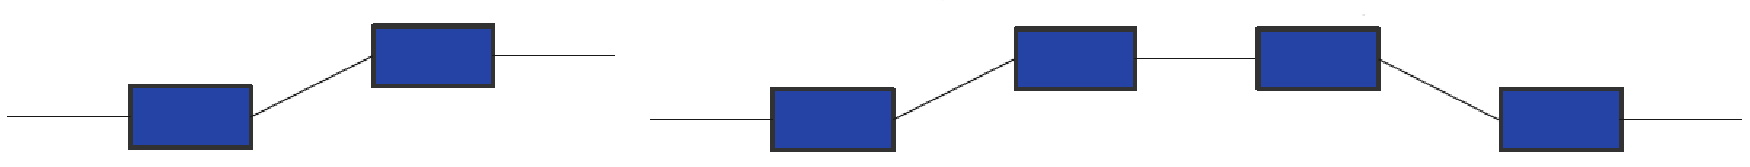
\includegraphics[width=\textwidth]{Figures/Energy_Recovery_Linac_Design/chicane_dogleg.pdf}
\caption{Lattice schematics with dipoles (blue) and drifts (black, line). Left: Dogleg lattice. Right: Chicane lattice. }
\label{fig:chicane_dogleg_schematic}
\end{figure}

The dogleg therefore has a transport matrix of the form
\begin{equation}
\boldsymbol{R}_{\mathrm{dog}} = \boldsymbol{R}_{\mathrm{dip,2}}\cdot\boldsymbol{R}_{\mathrm{drift}}\cdot\boldsymbol{R}_{\mathrm{dip,1}},
\label{eq:dogleg_transport_matrix_simple}    
\end{equation}
which yields 
\begin{equation}
\resizebox{\columnwidth}{!}{
\boldsymbol{R}_{\mathrm{dogleg}} = 
\begin{pmatrix}
1+\frac{L}{\rho}\cos\alpha_{1}\sin\alpha_{1} & L_{\mathrm{drift}}\cos^{2}\alpha_{1} & 0 & 0 & 0 & -L_{\mathrm{drift}}\cos\alpha_{1}\sin\alpha_{1} \\
-\frac{L_{\mathrm{drift}}}{\rho^{2}}\sin^{2}\alpha_{1} & 1-\frac{L_{\mathrm{drift}}}{\rho}\cos\alpha_{1}\sin\alpha_{1} & 0 & 0 & 0 \frac{L_{\mathrm{drift}}}{\rho}\sin^{2}\alpha_{1} \\
0 & 0 & 1 & L_{\mathrm{drift}}+2\rho\alpha_{1} & 0 & 0 \\
-\frac{L}{\rho}\sin^{2}\alpha_{1} & -L_{\mathrm{drift}}\sin\alpha_{1}\cos\alpha_{1} & 0 & 0 & 1 & L_{\mathrm{drift}}\left(1+\sin^{2}\alpha_{1}\right) \\
0 & 0 & 0 & 0 & 0 & 1
\end{pmatrix}
\label{eq:6D_dogleg_matrix}}    
\end{equation}
where the path length of the dogleg is $L=L_{\mathrm{drift}}+2L_{\mathrm{dip}}$ and the $\boldsymbol{R}_{56}$ matrix element is given by
\begin{equation}
\boldsymbol{R}_{56} = L_{\mathrm{drift}}\left(1+\sin^{2}\alpha_{1}\right),
\label{eq:dogleg_R56}    
\end{equation}
therefore $\boldsymbol{R}_{56}>0$ for a dogleg lattice. In the longitudinal co-ordinates ($z$,$\Deltap/p_{0}$), the transformation from the particles entrance to the dogleg ($z_{0}$, $\left(\Delta p/p_{0}\right)_{0}$) to its exit ($z_{1}$, $\left(\Delta p/p_{0}\right)_{1}$) yields the relations
\begin{align}
z_{1} &= z_{0}+\boldsymbol{R}_{56}\left(\frac{\Delta p}{p_{0}}\right)_{0} = z_{0} + L_{\mathrm{drift}}\left(1+\sin^{2}\alpha_{1}\right)\left(\frac{\Delta p}{p_{0}}\right)_{0}, \\
\left(\frac{\Delta p}{p_{0}}\right)_{1} &= \left(\frac{\Delta p}{p_{0}}\right)_{0} = \frac{\Delta p}{p_{0}},
\label{eq:longitudinal_dogleg_transform}    
\end{align}
where the momentum spread is, as expected, unchanged and throughout the dogleg lattice the bunch will be longitudinally spread by a factor $\Delta z=\boldsymbol{R_{56}}\frac{\Delta p}{p_{0}}$.

Similarly, a chicane bunch compressor can be constructed from a dogleg and a reverse dogleg (the reflection of the dogleg shown in Fig.~\ref{fig:chicane_dogleg_schematic}) separated by a drift. The path length of this chicane is $L = 4L_{\mathrm{dip}}+2L_{\mathrm{drift,1}}+L_{\mathrm{drift,2}}$, where each dipole is of identical length and $L_{\mathrm{drift,1}}\neq L_{\mathrm{drift,2}}$. The resulting lattice is shown in Fig.~\ref{fig:chicane_dogleg_schematic}. 

The transport matrix of this lattice is of the form
\begin{equation}
\boldsymbol{R}_{\mathrm{chicane}} = \boldsymbol{R}_{\mathrm{dip,2}}\cdot\boldsymbol{R}_{\mathrm{drift,1}}\cdot\boldsymbol{R}_{\mathrm{dip,1}}\cdot\boldsymbol{R}_{\mathrm{drift,2}}\cdot\boldsymbol{R}_{\mathrm{dip,1}}\cdot\boldsymbol{R}_{\mathrm{drift,1}}\cdot\boldsymbol{R}_{\mathrm{dip,2}},
\label{eq:chicane_transport_matrix}    
\end{equation}
where, for brevity, the full 6D transport matrix is not shown. The $\boldsymbol{R}_{56}$ matrix element of the chicane becomes
\begin{equation}
\boldsymbol{R}_{56} = -2L_{\mathrm{drift,1}}\frac{\alpha_{1}\sin\alpha_{1}}{\cos^{2}\alpha_{1}},
\label{eq:chicane_R56}    
\end{equation}
therefore, $\boldsymbol{R}_{56}<0$ for a chicane. The longitudinal co-ordinates transform in a chicane such that
\begin{align}
z_{1} &= z_{0} + \boldsymbol{R}_{56}\left(\frac{\Delta p}{p_{0}}\right)_{1} = z_{0} + 2L_{\mathrm{drift,1}}\frac{\alpha_{1}\sin\alpha_{1}}{\cos^{2}\alpha_{1}}\left(\frac{\Delta p}{p_{0}}\right), \\
\left(\frac{\Delta p}{p_{0}}\right)_{1} &= \left(\frac{\Delta p}{p_{0}}\right)_{0} = \frac{\Delta p}{p_{0}}. 
\label{eq:longitudinal_chicane_transform}    
\end{align}

As proven for a dogleg (Eq.~\ref{eq:longitudinal_dogleg_transform}), the chicane transform has a similar form with unchanged momentum variation and a variation in the longitudinal co-ordinate of $\Delta z = \boldsymbol{R}_{56}\frac{\Delta p}{p_{0}}$, which here is a compression due to $\boldsymbol{R}_{56}<0$.

Upon examination of the momentum compaction factor (Eq.~\ref{eq:momentum_compaction_first_order}), the path length variation can be re-cast using the longitudinal relationship \cite{wolski2012longitudinal} derived in the chicane (Eq.~\ref{eq:longitudinal_chicane_transform}) and dogleg (Eq.~\ref{eq:longitudinal_dogleg_transform}) examples yielding 
\begin{equation}
\alpha_{p} = \frac{\boldsymbol{R}_{56}}{L},
\label{eq:momentum_compaction_R56}
\end{equation}
which can be used to re-define the $\boldsymbol{R}_{56}$ using (Eq.~\ref{eq:momentum_compaction_dispersion})
\begin{equation}
\boldsymbol{R}_{56} = \int_{0}^{s}\frac{\eta_{x}}{\rho}ds.    
\label{eq:R56_dispersion_relation}
\end{equation}

Many other types of bunch compression devices can be designed such as arc-like bunch compressors \cite{williams2020arclike} with $\boldsymbol{R}_{56}>0$ , and the introduction here is not intended to be comprehensive. 

\section{Linear Transport Lattices}

Transport lattices for accelerators typically consist of repeated cells, to produce periodic motion of the accelerated particles, these repeated cells differ in design based on the desired beam properties in each case. However, magnetic lattices for particle accelerators can come in many forms and designs, therefore a comprehensive review is beyond the scope of this thesis. Consequently, A review of the cell structure of the linear transport lattices most relevant to ERL design and the work in further chapters is pursued here via three lattice types: the FODO lattice, a multi-bend achromat and the fixed field alternating gradient (FFA) approach. 

\subsection{FODO Lattice}
\label{sec:FODO_lattice}

A FODO lattice consists of a series of alternatively focusing quadrupoles separated by drifts as shown in Fig.~\ref{fig:FODO_cell}. The FODO lattice aims to provide periodic focusing, which requires that the Twiss parameters remain unchanged from the entrance to exit of the cell. For simplicity, thin lens quadrupoles (Eq.~\ref{eq:quadrupole_matrix_thin}) are considered, the dynamics is limited to the $x$--$x'$ phase space plane and the focusing fields are considered to be of equal magnitude.

\begin{figure}[!h]
\centering
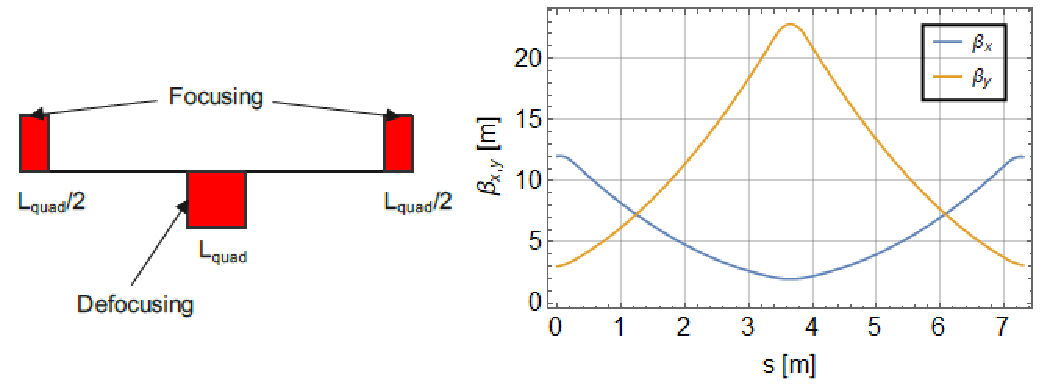
\includegraphics[width=\textwidth]{Figures/Energy_Recovery_Linac_Design/FODO_cell_finished.pdf}
\caption{Left: FODO cell schematic. Alternating focusing quadrupole (red) arrangements, separated by drifts of length $L_{\mathrm{drift}}$. Focusing quadrupoles of length $L_{\mathrm{quad}}/2$ and defocusing quadrupole of length $L_{\mathrm{quad}}$. Right: $\beta$-functions in each plane of a FODO cell created using \textsc{Tao} \cite{TaoManual}.}
\label{fig:FODO_cell}
\end{figure}

The FODO cell has a transport matrix of the form
\begin{equation}
\boldsymbol{R}_{\mathrm{FODO}} = \boldsymbol{R}_{\mathrm{quad,F}}\cdot\boldsymbol{R}_{\mathrm{drift}}\cdot\boldsymbol{R}_{\mathrm{quad,D}}\cdot\boldsymbol{R}_{\mathrm{drift}},
\label{eq:FODO_transport}    
\end{equation}
where the $x$--$x'$ plane transport matrices are
\begin{align}
\boldsymbol{R}_{\mathrm{quad,F}} &= 
\begin{pmatrix}
1 & 0 \\
-\frac{1}{f} & 0
\end{pmatrix}, & \boldsymbol{R}_{\mathrm{quad,D}} &= 
\begin{pmatrix}
1 & 0 \\
\frac{1}{f} & 1
\end{pmatrix}, & \boldsymbol{R}_{\mathrm{drift}} &= 
\begin{pmatrix}
1 & \frac{L}{2} \\
0 & 1
\end{pmatrix},
\label{eq:FODO_component_matrices}    
\end{align}
such that the transport matrix for a FODO cell becomes
\begin{equation}
\boldsymbol{R}_{\mathrm{FODO}} =
\begin{pmatrix}
1+\frac{L}{2f} & L+\frac{L^{2}}{4f} \\
-\frac{L^{2}}{4f} & 1-\frac{L}{2f}-\frac{L^{2}}{4f}
\end{pmatrix}.
\label{eq:FODO_matrix}
\end{equation}
Through using the general matrix of periodic transport (Eq.~\ref{eq:periodic_transport_matrix}) for a single turn, we can relate the phase advance $\mu$ to the parameters of the FODO cell
\begin{align}
\cos\mu &= \frac{1}{2}\boldsymbol{\mathrm{Tr}}\left(\boldsymbol{R}_{\mathrm{FODO}}\right) = 1-\frac{L^{2}}{8f^{2}}, \\
\cos\mu &= 1-2\sin^{2}\left(\frac{\mu}{2}\right), \\
\left|\sin\left(\frac{\mu}{2}\right)\right| &= \frac{L}{4f}.
\label{eq:phase_advance_FODO}
\end{align}
Using the previously defined stability criterion (Eq.~\ref{eq:stability_criterion}), the FODO cell is therefore only stable under the condition
\begin{equation}
1>\frac{L}{4f},
\label{eq:FODO_stability}    
\end{equation}
which for a typical phase advance $\mu=90$\si{\degree}, means the focal length is given by
\begin{equation}
f=\frac{L}{2\sqrt{2}}.
\label{eq:FODO_focal_90}    
\end{equation}

\subsection{Multi-Bend Achromat}

An achromat lattice has cells in which the dispersion of the particle beam is zero at the entrance and exit of the lattice cell, whilst bending occurs in the central portion of the cell. In the simplest form -- known as a double bend achromat -- a single quadrupole focusing magnet is placed between two dipoles where additional quadrupoles are placed outside of this central region to maintain periodic focusing, as in the FODO cell in Section~\ref{sec:FODO_lattice}. The central section of a double bend achromat and the corresponding dispersion function are shown in Fig.~\ref{fig:DBA_diagram}.

\begin{figure}[!h]
\centering
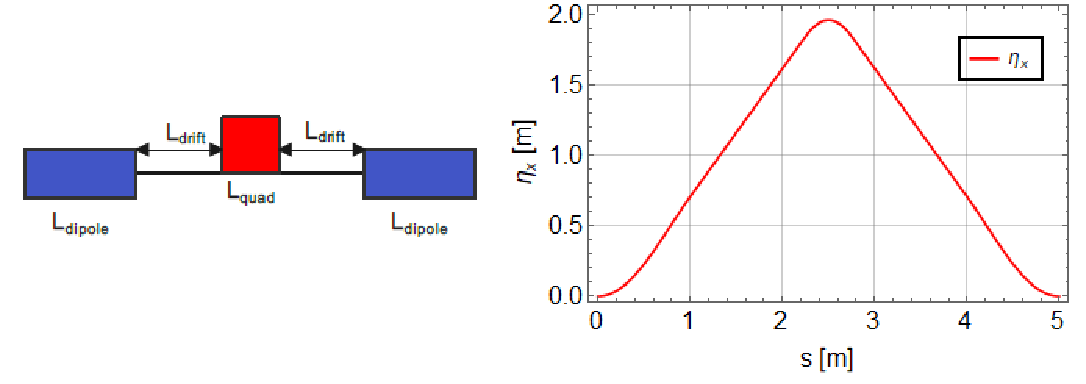
\includegraphics[width=\textwidth]{Figures/Energy_Recovery_Linac_Design/DBA_diagram.pdf}
\caption{Left: Cell central region of double bend achromat, consisting of a a quadrupole (red) of length $L_{\mathrm{quad}}$ placed between two dipoles (blue) of length $L_{\mathrm{dipole}}$ with magnets separated by drift $L_{\mathrm{drift}}$. Right: Dispersion function $\eta_{x}$ in the $x$ plane $\eta_{x}$ as a function of longitudinal distance $s$. Dispersion peaks within the centre of a DBA and is zeroed at the start and end of the central section of a DBA created using \textsc{Tao} \cite{TaoManual}}
\label{fig:DBA_diagram}
\end{figure}

The requirement of zero dispersion as the entrance and exit of the double bend achromat cell means that the required magnet strengths can be derived from (Eq.~\ref{eq:periodic_dispersion}), with $\eta_{x,0}=0$.
A full derivation is beyond the scope of this thesis, but is shown by Steffen \cite{steffen1983periodic} and Fakhiri et al \cite{fakhri2015analytical} to be
\begin{equation}
\frac{1}{\sqrt{k_{1}}}\cot\left(\frac{\sqrt{k_{1}}L_{\mathrm{quad}}}{2}\right) = L_{\mathrm{drift}} + \rho\tan\left(\alpha_{1}/2\right),
\label{eq:DBA_magnets}
\end{equation}
where $k_{1}$ is the normalised quadrupole gradient, $L_{\mathrm{quad}}$ is the magnetic length of the quadrupole with $\rho$ and $\alpha_{1}$ the bending radius and bending angle of the dipoles respectively. 

The order $n$ of the achromat can be extended by replacing the central achromat section with $n$ dipoles with at least a single quadrupole between each yielding $n-1$ minimum quadrupoles. This generalistion can be followed to the $n$th order where the lattice structure is named a multi-bend achromat (MBA). Benefits to higher order achromats involve the avoidance of tune resonances, due to the decoupling of constraints on tune, lower emittance, potentially smaller dispersion peaks and generally a more flexible transport lattice \cite{jackson1986comparison} at the cost of an increased number of magnets and potentially larger circumference.  

\subsection{Fixed Field Alternating Gradient}
\label{sec:FFA}

Fixed field alternating gradient transport is designed using constant field magnets, like cylotrons, with alternating gradient focusing, like synchrotrons \cite{machida2013fixed}. The magnet fields are not varied in order to account for higher energies, instead the lattice is designed such that varying momentum particles are contained within tolerable displacements from the reference orbit. FFA transport is particularly advantageous due to the high momentum variation, or acceptance, that the lattice can tolerate, as in an FFA an orbit can be defined at any particle momentum \cite{barlow2010emma}. There are two forms of FFA transport: scaling and non-scaling, which relate to the relationship between the magnetic field gradient of the magnets and the radial position of a magnet.

In a scaling FFA the main design consideration is to keep the tune of the orbit constant with respect to energy to avoid optical resonances via crossing integer tunes \cite{symon1956fixed}. Constant tune is satisfied by having geometrically similar magnetic fields for different energies $E$ and orbital radii $R$ ($E\propto R$), which can be expressed by
\begin{equation}
\left.\frac{\partial}{\partial p} \left(\frac{\rho}{\rho_{0}}\right)\right|_{\alpha_{1}=\mathrm{const}}=0,
\label{eq:scaling_condition}    
\end{equation}
where $\rho$ is the local radius of curvature and $\rho_{0}$ is the average radius of curvature. The scaling condition (Eq.~\ref{eq:scaling_condition}) is satisfied by magnetic field profiles for two varying designs: a radial sector FFA (Eq.~\ref{eq:radial_FFA_field}) and a spiral sector FFA (Eq.~\ref{eq:spiral_FFA_field}) of the form \cite{symon1956fixed}
\begin{align}
B &= B_{0}\left(\frac{r}{r_{0}}\right)^{k}, 
\label{eq:radial_FFA_field} \\
B &= B_{0}\left(\frac{r}{r_{0}}\right)^{k}\left\{1+f\cos\right[N\alpha_{1}-N\tan\left(\zeta\right)\log\left(\frac{r}{r_{0}}\right)\left]\right\},
\label{eq:spiral_FFA_field}
\end{align}
where generally, $r$ is the radial distance from the centre of the accelerator and $k$ is the field index
\begin{equation}
k=-\frac{r_{0}}{B_{z}\left(r_{0}\right)}\left(\frac{\partial B_{z}}{\partial r}\right)_{r=r_{0}},
\label{eq:FFAG_field_index}
\end{equation}
and, applying to spiral sector FFA, $f$ is the flutter factor, $N$ the number of sectors and $\zeta$ the spiral angle between the locus of the maximum field and the radius. Variation between the scaling FFA designs is not investigated here as the focus is on non-scaling FFA; a further discussion of scaling FFA is presented by Symon et al \cite{symon1956fixed}. However, we note that the scaling FFA design is limited as it is constrained by constant tune to obey the scaling condition (Eq.~\ref{eq:scaling_condition}), which limits the flexibility of the optics, can only be satisfied by complicated magnets with specific field profiles (Eqs.~\ref{eq:radial_FFA_field}, \ref{eq:spiral_FFA_field}) and requires a large radius accelerator for high energy electrons. The alternative is non-scaling FFA lattices, in which the scaling condition (Eq.~\ref{eq:scaling_condition}) is disobeyed.

Once the scaling condition is not met, phase advance varies with momentum and the tune of the accelerator can cross an optical resonance, however resonance crossing may be tolerable for rapid crossings as the blow-up of the beam size may be limited \cite{mills1997nsffa,johnstone1997nsffa}. Therefore, the scaling FFA condition may be abandoned with rapid crossing of the optical resonances, and the working point of the transport optics can be allowed to vary. This has been demonstrated in simulation, where it was found that random dipole and quadrupole kicks were responsible to a greater extent for orbit distortion than optical resonance crossing \cite{machida2007orbit}. Removal of the scaling condition allows the radial variation of the magnetic field to be simplified to a linear relationship \cite{johnstone1999fixed}, hence complicated magnet design is no longer required and linear magnets are sufficient for non-scaling FFA transport.

A proof-of-principle demonstration of non-scaling FFA was performed with the EMMA accelerator \cite{barlow2010emma,machida2012acceleration}, and transport involving non-scaling FFA has been demonstrated at the CBETA ERL \cite{hoffstaetter2017cbeta,bartnik2020cbeta} with subsequent designs for accelerator driven sub-critical reactors \cite{tygier2011high} and radiotherapy gantries \cite{trbojevic2009ffags,} based on such an approach. Linear non-scaling FFAG transport typically consists of a lattice made of many cells in which two focusing magnets, are separated by drifts. Typically linear non-scaling FFA can be accomplished using at least one combined function magnet (bending and focusing) with a quadrupole or combined function magnet, where quadrupoles with transversely shifted pole centres are often utilised. An example non-scaling FFA cell is shown in Fig.~\ref{fig:FFA_cell}.

\begin{figure}[!h]
\centering
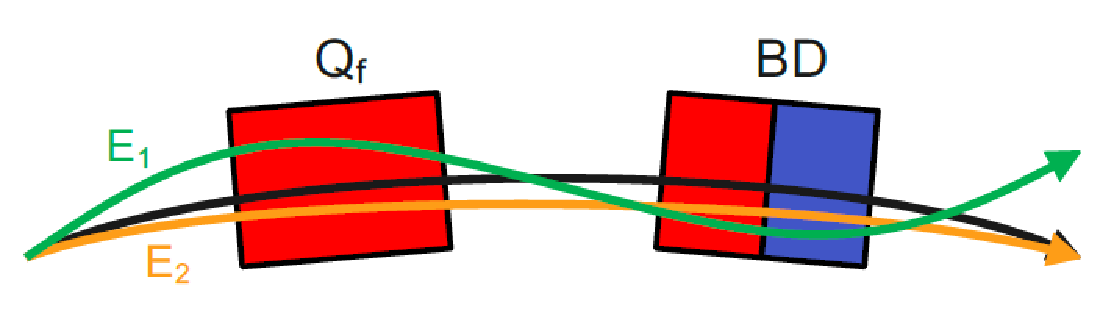
\includegraphics[width=0.7\textwidth]{Figures/Energy_Recovery_Linac_Design/FFA_cell_fixed.pdf}
\caption{Schematic of a FFA cell containing a focusing quadrupole $Q_{\mathrm{f}}$ (red) and combined function magnet $BD$ (blue and red), with reference trajectory (black). Particles with varying energies $E_{1}$ (green) and $E_{2}$ (orange) traverse the cell with varying trajectories.}
\label{fig:FFA_cell}
\end{figure}

\section{Energy Recovery Linacs}
\label{sec:ERL_theory}

An energy recovery linac is a form of re-circulated accelerator, invented by Tigner \cite{tigner1965possible} and first demonstrated at Stanford \cite{smith1987development}, which is capable of providing the high-quality particle bunch properties of a linac with the high duty factor (bunch repetition rate) of a storage ring. Characteristically, in an ERL the energy used to accelerate a particle bunch is recovered by the accelerating structure upon deceleration of the bunch when it is re-circulated and returned to the accelerating structure. The energy recovery linac scheme has numerous advantages which will be presented in this section whilst possible designs and considerations of ERLs are explained with a focus on electron machines. A full review of current and past ERL projects is not shown here and is instead used to contextualise the CBETA ERL in Chapter~\ref{CBETA_Multi-Pass_Commissioning}. 

\subsection{Single Turn ERL}
\label{sec:single_turn_ERL}
% description of a simple 1 turn 1 linac ERL
% ADV: Dumping beam at low energy + neutron threshold
% Turn + Passes definition
% Requirement of a phase change
% Next accelerated bunch benefits from the energy dumped
% Same cell energy recovery 
% DIAGRAM

Firstly, we consider a single turn energy recovery linac with a single electron bunch, which consists of a high repetition rate, high-brightness (low emittance, high bunch charge) photo-injector \cite{ben2016superconducting} and injection beamline, a linac section containing several RF cavities, a re-circulating transport beamline from the exit of the linac to its entrance and a beam dump. A schematic off the simplest form of single turn ERL is shown in Fig~\ref{fig:ERL_schematics}. 

\begin{figure}[!h]
\centering
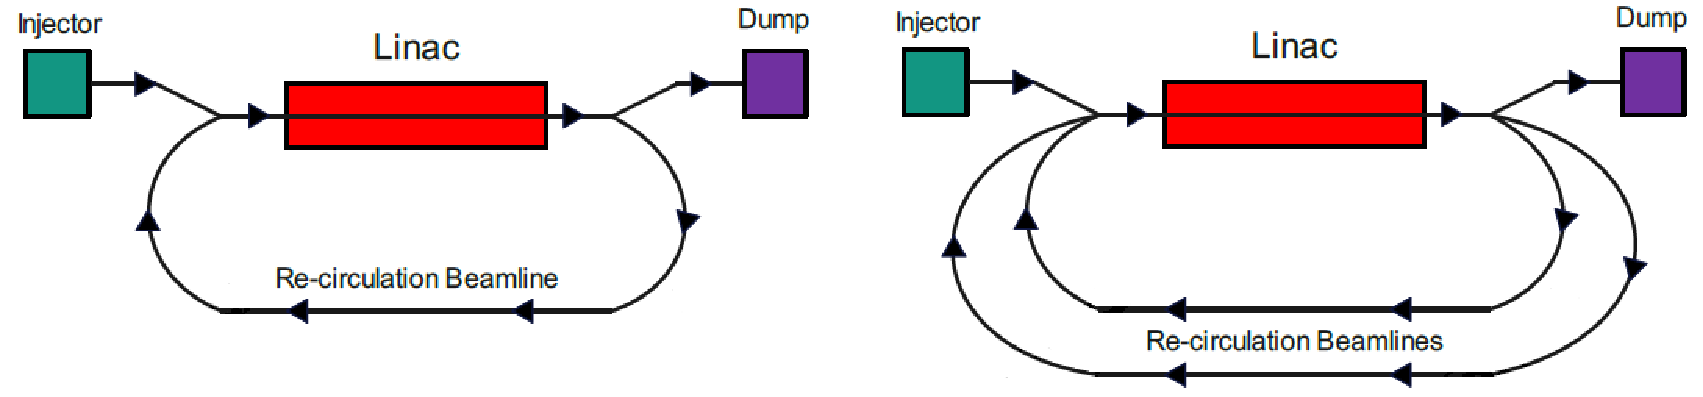
\includegraphics[width=\textwidth]{Figures/Energy_Recovery_Linac_Design/single_multi_turn_ERL.pdf}
\caption{Energy recovery linac diagrams showing the photo-injector (green), linac (red), beam dump (purple) and re-circulation beamline (black). Left: Single turn ERL. Right: Two Turn ERL with common transport (1st turn acceleration and deceleration transported in same beamline). }
\label{fig:ERL_schematics}
\end{figure}

Within the single turn ERL, the electron bunch is generated via the photo-injector at some kinetic energy $E_{\mathrm{inj}}$ and transported to the linac, where its arrival is timed to an accelerating phase of the RF waveform (see Section~\ref{sec:RF_acceleration}), as shown in Fig.~\ref{eq:ERL_RF_acceleration_phase}. The electron bunch is consequently accelerated to some kinetic energy $E_{e}$ and is transported via the re-circulating transport beamline until at the entrance to the linac. Upon re-entry into the linac, the electron bunch is decelerated and must be timed to a decelerating phase of the RF waveform -- a trough in the RF waveform. 

\begin{figure}[!h]
\centering
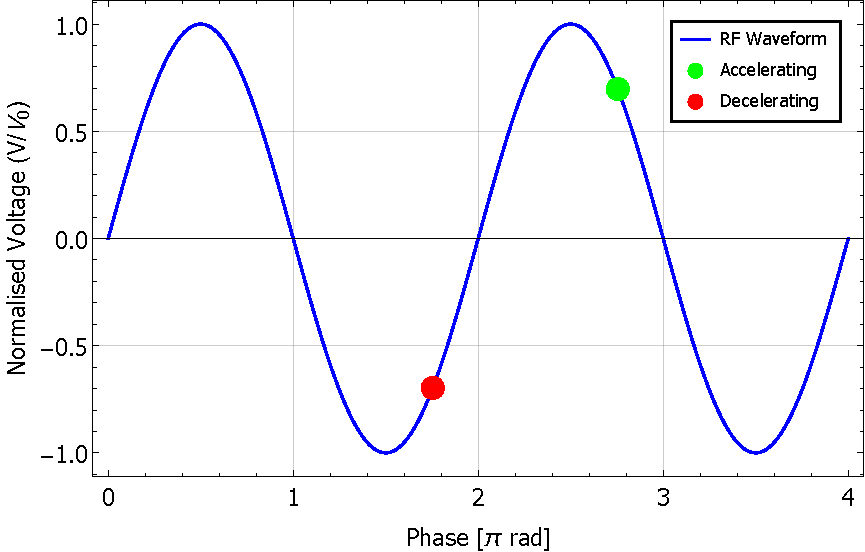
\includegraphics[width=0.7\textwidth]{Figures/Energy_Recovery_Linac_Design/ERL_acc_deacc_RF_phase.pdf}
\caption{Normalised RF voltage as a function of phase in an RF cavity. A phase suitable for off-crest acceleration (green) is shown, where phase focusing would occur ($\eta_{p}>0$, see Fig.~\ref{fig:phase_focusing_above_transition}), with its corresponding 180\si{\degree} varied defocusing phase (red).}
\label{eq:ERL_RF_acceleration_phase}
\end{figure}

For a decelerating phase at the linac re-entrance the phase must be altered by 180\si{\degree} by configuring the path length of the re-circulating transport line to have a path length of $L= \lambda_{\mathrm{RF}}\left(n+\frac{1}{2}\right)$ i.e some integer $n$ RF wavelengths plus half an RF wavelength (for the 180\si{\degree} phase change), as shown in Fig.~\ref{eq:ERL_RF_acceleration_phase}. The electron bunch is then decelerated to a kinetic energy $E_{\mathrm{inj}}$ and the energy from the decelerated bunch is transferred to the RF cavity for acceleration of the next particle to traverse the accelerating structure. When the energy of the electron bunch is transferred, via deceleration, to the same RF cavity that accelerated the bunch this is termed same cell energy recovery, however more elaborate systems are possible. The electron bunch is then transported to the beam dump. In our convention, the electron bunch has undergone a single turn but passes the linac twice.

Through the simplistic description of a single turn ERL it is clear that there are numerous advantageous features. Firstly, the electron bunch in the dump has been decelerated to $E_{\mathrm{inj}}$, avoiding the necessity of a high-energy beam dump and, if this is below $\sim10$~\si{\mega\electronvolt}, neutron activation of the dump may be avoided. The energy required to accelerate the electron bunch is returned to the RF cavities for acceleration of a future bunch meaning that the beam power of the electron bunch is not lost and the RF system efficiently accelerates electron bunches. Also, as the bunch is dumped after a single turn, the electron bunch emittance  has not equilibriated -- as in a storage ring \cite{owen2013nonequilibrium} -- and is replaced, at a high repetition rate, by another electron bunch. Therefore, from an ERL, small emittances are achievable at high repetition rate -- the advantageous facets of both a linac and storage ring -- with the additional bonus of an efficient RF system, without the necessity of a high energy beam dump. 

\subsection{Multi-Turn ERL}
\label{sec:multi_turn_ERL}
% Accelerating phase condition + re-circulated linacs
% ADV: reach high energy with small RF outlay
% relations between no. passes + turns
% merger + splitter sections
% complexity introduced due to many varying energy beams and therefore transport considerations
% DIAGRAM

Multi-turn ERLs are similar to the single turn ERL, however a multi-turn ERL takes advantage of multiple accelerations by the RF cavity. As an example, consider a 2 turn ERL with a single linac accelerating section, a photo-injector and beam dump as well as 2 re-circulating beamlines. A schematic of this simple 2 turn ERL is shown in Fig.~\ref{fig:ERL_schematics}.  

The electron bunch is generated via the photo-injector with energy $E_{\mathrm{inj}}$ and transported to the linac, arriving with accelerating phase, and is accelerated with energy gain $\DeltaE$ (Eq.~\ref{eq:particle_energy_gain_RF}) to a kinetic energy $E_{e,1}$, the first turn nominal energy. The electron bunch is then transported to the entrance of the linac, via the first re-circulating beamline, in accelerating phase and is re-accelerated to $E_{e,2}=2\Delta E+E_{\mathrm{inj}}$, an increased second turn nominal energy. For acceleration, the first re-circulating beamline must have a path length of $L = n\lambda_{\mathrm{RF}}$ to return to the same phase as the initial acceleration. The scheme thus far is identical to a re-circulating linac machine first demonstrated at MUSL-2 \cite{axel1977status}.

The electron bunch then enters the second re-circulating beamline which re-circulates the electron bunch to the entrance of the linac. The second re-circulating beamline must conduct the 180\si{\degree} phase change and therefore the path length is of the form $L=\lambda_{\mathrm{RF}}\left(n+\frac{1}{2}\right)$. On the third pass of the linac the electron bunch is decelerated to $E_{e,1}$, and is subsequently transported around the first recirculating beamline with path length of the form $L=n\lambda_{\mathrm{RF}}$, which maintains the decelerating phase of the electron bunch upon arrival at the entrance to the linac for the 4th pass. The 4th pass of the linac decelerates the electron bunch from $E_{1}$ to $E_{\mathrm{inj}}$, which is subsequently transported to the beam dump. Therefore, a single linac 2 turn ERL consists of 4 linac passes and 3 traversals of a re-circulating beamline; in general a $n$ turn ERL requires $2n$ linac passes and $2n-1$ traversals of a re-circulating beamline.

A multi-turn ERL is advantageous over a single turn ERL as, with a limited accelerating section, a high electron bunch kinetic energy can be achieved via multiple passes. All advantages of the single turn ERL are also maintained. However, with multiple nominal energies existing within the ERL, transport design is more complex in the multi-turn ERL with multiple re-circulation beamlines which all need to pass through the same linac leading to the development of complex, magnet dense transport sections named spreader sections which direct different nominal energy electron beams through the reference orbit of the linac. Re-circulation of the electron bunch is further complicated by the need to transport both an accelerating and decelerating bunch of identical nominal energy which results in the need to have a single beamline that satisfies the transport conditions of both accelerating and decelerating bunches, as in the example described above, or transport these in separate beamlines. The discussion of transport options for ERLs is furthered in Section~\ref{sec:ERL_transport_options} 

\subsection{ERL Transport Options}
\label{sec:ERL_transport_options}
% Single Transport
% Common Transport
% Multi-energy Common Transport

The multi-turn ERL has three main possible forms of transport design: single transport, common transport and multi-energy common transport, which are explained within this section. Transport in ERLs is subject to many constraints such as the path length condition for acceleration, typical transport matching considerations (beam optics matching, momentum acceptance etc.) and, dependent on the experimental requirements of users, any interaction region or insertion device constraints -- like the final focus systems of ICS sources investigated in this thesis. Therefore, the ERL transport options are also evaluated on their applicability in the situation of ERL driven radiation generation (ICS, FEL) as well as their general properties.

Conceptually, the simplest transport design for the multi-turn ERL is single transport, where each accelerating and decelerating pass of the linac (at each nominal turn energy) is transported by a dedicated re-circulating beamline. There are $2n-1$, where $n$ is the no. turns, re-circulating beamlines in the ERL. As the constraints for the bunch are only satisfied for a single bunch configuration in each beamline single transport benefits from the most flexible optics. Less constrained optics allow for an integrated interaction region for radiation experiments etc. which can be more easily imposed. 

However, with $2n-1$ recirculating beamlines the quantity of magnets required is vast, adding additional cost into a design. During acceleration and deceleration bunches must traverse the axis of the linac, therefore complex beamline regions -- named spreader/recombiners -- are required to make all turns traverse the linac axis. Consequently, spreaders are typically spatially complex beamline designs with many nearby magnets. Nearby magnets mean beamlines can be subject to the fields generated in neighbouring beamlines, creating a cross-talk between passes.

Common transport design, shown for the 2 turn ERL in Fig~\ref{fig:ERL_schematics}, uses identical beamlines for accelerating and decelerating passes therefore $n-1$ re-circulating passes are required. In a multi-turn ERL, the $n$th pass is traversed a single time by the highest kinetic energy bunch in a decelerating configuration whereas each other re-circulating beamline is traversed twice (accelerating and decelerating). Consequently, a dedicated beamline can be constructed for the required 180\si{\degree} phase change from acceleration to deceleration.

The common transport requirement for $n-1$ beamlines (in contrast to single transports $2n-1$ beamlines), reduces the complexity of spreader/recombiner designs and theoretically requires less accelerator magnets. Yet, the individual re-circulating beamlines must satisfy the constraints of two passes and are less adjustable (more constrained). Correction of the transport optics becomes more difficult as any correction affects both the accelerating and decelerating traversal. Design of interaction regions for radiation generation also becomes more difficult as at the interaction point both acceleration and decelerating bunches must have identical properties as radiation generation is sensitive to the bunch distribution, further constraining the optics.

Common transport design can be extended such that a single beamline transports each energy -- termed multi-energy common transport -- where all nominal beam energies, in both accelerating and decelerating configuration, are transported by the same re-circulating beamline. Only a single beamline is required, constructed of optics able to transport multiple varying energy beams -- such as the non-scaling FFA in Section~\ref{sec:FFA}. The single re-circulating beamline is highly constrained and orbits must be designed to accommodate for the path length variation (180\si{\degree} RF phase change) required in the $n$th pass, to satisfy all optical matching conditions and allow for on-axis linac traversal. 

When all constraints can be satisfied in the single re-circulating beamline, spreader/recombiner systems are not required. However, a fully multi-energy common transport multi-turn ERL scheme has not been demonstrated -- the CBETA ERL \cite{hoffstaetter2017cbeta,bartnik2020cbeta} which uses multi-energy common transport uses common transport spreader designs to provide additional path length correction and linac matching. The number of accelerator magnets required can also be reduced, however optics like non-scaling FFA are magnet dense.

Correction of multi-energy common transport systems is difficult as variation in any magnet affects all $2n-1$ passes of the re-circulating beamline. Considering the use of a multi-turn common transport system for radiation production there are several issues; the lattices are magnet dense so incorporating an interaction region is difficult and interaction region design is not easily adjustable, with bunches requiring different focusing and off-orbit trajectories for particles in FFA. The constraints on the design of an interaction region in a multi-energy common transport system are increased $2n-1$ fold from the single transport case.   

\subsection{High Current ERL Operation}
\label{sec:high_current_ERL}
% Beam current limitations
% Continuous wave operation vs pulsed
% normal vs superconducting RF

Operating with high current is advantageous for an ERL as high current will allow for delivery of a large number of particles to users of the accelerator; beneficial in both colliders and radiation generating light sources -- two touted applications of ERLs. However, the current can be limited in numerous ways, for example by operating in a pulsed mode with a series of bunch trains or due to collective effects such as beam breakup instability. 

Within an ERL, the bunch generation can occur in two modes of operation: pulsed beam or continuous wave (CW) operation. In pulsed beam operation a series of bunches are generated and accelerated in a bunch train, with a pause before another bunch is generated. In continuous wave operation bunches are continually generated and accelerated with all RF buckets of the accelerator filled which means a higher current can be achieved. Additionally,
creation of a very stable beam (in energy) and very low energy spread
is easier with CW resonant systems rather than pulsed systems \cite{reece2016continuous}. However, high acceleration gradients are required for high energy ERL operation to reduce the footprint of the ERL but have large power consumption during CW operation. Continuous wave acceleration gradients of above 5~\si{\mega\volt}/\si{\meter} are not sustainable with normal conducting accelerating structures \cite{reece2016continuous} as resistive wall losses become challenging thermally, and the associated required power becomes infeasible. Therefore, for high energy ERLs with CW operation superconducting RF (SRF) structures are the most viable solution. 

The average beam current off energy recovery linacs can be limited by the effects of the beam breakup instability (BBU). In the beam breakup instability, the electron bunch interacts with a higher order mode (HOM) of the accelerating structure and is deflected. Electron bunches with a transverse offset traverse an RF cavity and excite a HOM within the cavity. The electron bunch subsequently receives a transverse kick, thereby generating a further higher order mode due to the transverse offset the kick generates. Beyond some threshold current value $I_{\mathrm{th}}$ this process becomes exponential in nature resulting in beam loss.

Two forms of beam breakup exist; cumulative BBU in which the instability builds up over a series of RF accelerating structures, for example a long (100's~\si{\meter}) linac, and regenerative BBU where the effect build up via multiple passes of the same RF cavity. The former of these was the observed first, with experimentation at SLAC \cite{panofsky1966electrons,altenmueller1966beam} and LLNL \cite{neil1970coherent} and analytically modelled by Panofsky and Bander et al \cite{panofsky1968asymptotic}. However, for ERLs -- especially multi-turn ERLs -- regenerative beam breakup instability is of greater concern due to the recirculated nature of the accelerator in which a short linac section is typical. Regenerative BBU is particularly present in multi-turn ERLs in comparison to circular machines such as synchrotrons because the multiple energy bunches in the ERL are deflected differently for the same HOM voltage causing variation in bunch transverse offsets and a change in revolution time for the first decelerating bunch, in which the phase is modulated by 180\si{\degree} \cite{setiniyaz2021filling}.

Theoretical studies of regenerative BBU in ERL's were conducted by Hoffstaetter and Bazarov \cite{hoffstaetter2004beam} for uncoupled optics, then furthered for the case of coupled optics \cite{hoffstaetter2007recirculating}. The focus is typically on the excitation of dipole higher order modes, as these are typically the easiest to excite. Experimentally, regenerative BBU was observed and studied in an ERL at the Jefferson Laboratory FEL \cite{tennant2005first,douglas2006experimental}. Conventional methods of suppressing BBU \cite{tennant2004methods} in an ERL include HOM dampeners, as well as accelerator optics based solutions \cite{rand1980beam}. Recently BBU studies have been performed for the CBETA ERL \cite{lou2019beam} which have predicted a restrictive average beam current limitation of $I_{\mathrm{th}} = 40$~\si{\milli\ampere}. However, mitigation of regenerative BBU remains an active field exemplified by the proposal of a bunch filling pattern which could increase the threshold current limitation by up to a factor of 5 for a 3-turn ERL \cite{setiniyaz2021filling}.    

High average current in ERLs is also limited by beam halo, in which a low density collection of particles is situated outside of the core of the particle bunch. Beam halo in ERLs can be generated by myriad factors, such as the design of optics, magnetic field errors and non-linearities as well as photo-cathode choice, the photo-injection system and vaccum issues such as residual gas scattering \cite{neil2006jlab,tanaka2018new}. Mitigation can be achieved through optics studies and correction as well as photo-cathode choice and design of RF accelerating structures, many of which are active areas of study. Beam halo provides challenges for high current operation as the beam halo particles can be lost within transport, producing radiation doses above safety limits and damaging sensitive components such as magnets. At high current the particle loss is increased and becomes intolerable.

\subsection{Dual Linac ERLs}
\label{sec:dual_linac_ERL}

So far, within Sections~\ref{sec:single_turn_ERL}, \ref{sec:multi_turn_ERL}, only the most simple ERL designs have been mentioned. Within this section dual linac ERLs are explored with two designs shown in Fig.~\ref{fig:dual_linac_ERL_designs}.

\begin{figure}[!h]
\centering
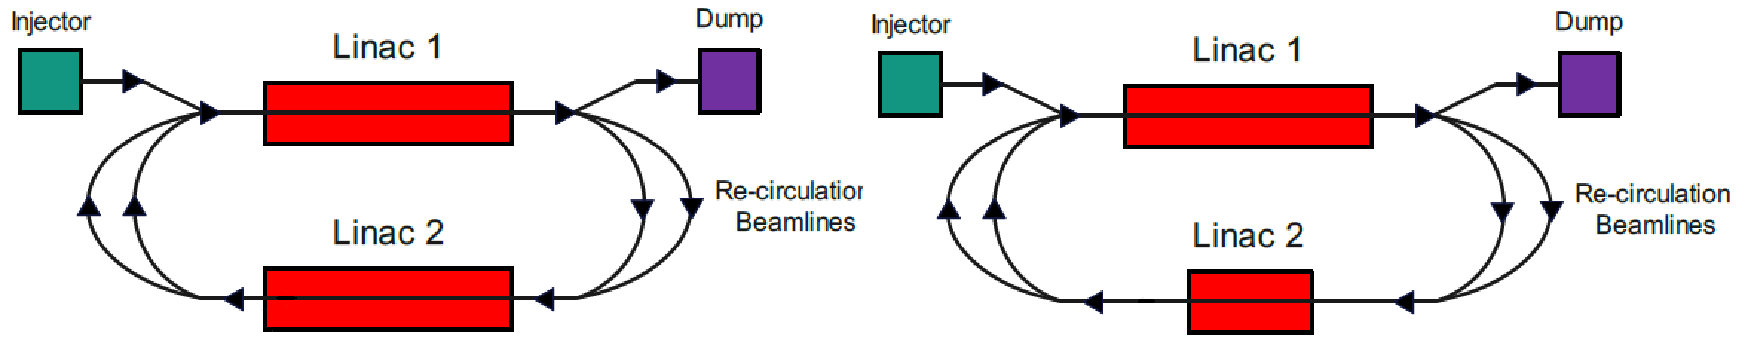
\includegraphics[width=\textwidth]{Figures/Energy_Recovery_Linac_Design/dual_linac_ERLs.pdf}
\caption{A series of alternative, more complex energy recovery linac design schematics. Basic components such as photo-injector (green), linac (red), beam dump (purple) and transport (black) are shown. Left: Symmetric dual linac ERL. Right: Asymmetric dual linac ERL.}
\label{fig:dual_linac_ERL_designs}
\end{figure}

In a symmetric dual linac ERL, the electron bunch is accelerated or decelerated twice by two separate linac passes on each pass of the machine -- there are $n$ turns, $2n-1$ passes and $2\left(n-1\right)$ traversals of linacs. A symmetric dual linac ERL has two identical linacs, which each provide half of the energy gain per turn meaning $2n$ nominal kinetic energies of the particles circulate from an $n$ turn ERL. Additional electron bunch energies may be beneficial to the design of a multi-colour light source from an ERL. Dual linacs also allow the size of the accelerating section to be shortened, since two linacs are utilised, which may provide an option for more compact high energy ERLs. Added complexity arises from the additional two sets of spreaders required for on-axis acceleration in the additional linac and from matching the additional phases for acceleration and deceleration. 

The dual asymmetric ERL offers similar flexibility and advantages to the symmetric dual linac ERL, but the kinetic energy of the accelerated particles does not increase uniformly step-wise. For example, with a total energy gain per turn of 50~\si{\mega\electronvolt}, a injection energy of $E_{\mathrm{inj}}=5$~\si{\mega\electronvolt} and a 2 turn ERL the energies available in the symmetric case per linac pass would be 30, 55, 80, 105~\si{\mega\electronvolt}. Whereas, a similar ERL but with a $4:1$ asymmetric linac energy gain ratio could provide energies 45, 55, 95, 105~\si{\mega\electronvolt}. Asymmetric linacs providing varying bunch kinetic energy may simplify spreader design, as the bend angles required in spreader septa would no longer be uniformly spaced.

\end{document}